% Addressing Is Not Free — paper assembly.
%
% CITATION-BY-ADDRESS RULE: every number in prose carries an inline comment giving its artifact
% path and decision-record section. A number without an address does not ship.
% Figures come from docs/paper/figures/make_figures.py, tables from make_tables.py; both read
% ONLY persisted artifacts. Nothing in this file is hand-entered data.
%
% NeurIPS ships a style file we do not vendor here; this preamble reproduces the single-column
% 10pt layout with the same margins so the draft reads at submission width.
\documentclass[10pt]{article}

\usepackage[letterpaper,margin=1.25in]{geometry}
\usepackage{amsmath,amssymb,amsthm}
\usepackage{booktabs}
\usepackage{longtable}   % Appendix E's table is taller than a page and must break across pages.
\usepackage{needspace}   % Appendix F's command list must not orphan its last item onto a new page.
\usepackage{graphicx}
\usepackage{microtype}
\usepackage[hidelinks]{hyperref}
\usepackage{caption}
\usepackage{enumitem}
\usepackage{xcolor}

\captionsetup{font=small,labelfont=bf}
\setlist{nosep,leftmargin=1.4em}

\newtheorem{theorem}{Theorem}
\newtheorem{proposition}{Proposition}
\theoremstyle{definition}
\newtheorem{remark}{Remark}

% Scope limits travel with the findings they scope (standing rule).
\newcommand{\scope}[1]{\smallskip\noindent\textit{Scope.} #1\smallskip}
% The four non-licenses appear wherever the reconciliation is cited.
\newcommand{\nonlicense}[1]{\noindent\textcolor{black!70}{\small #1}}

\title{\bf Addressing Is Not Free:\\ Factored Knowledge Storage and the\\
       Key-Discrimination Limit of Dense Models\\[0.35em]
       \large\normalfont\itshape A pre-registered measurement study}
% Author block sits under the title/subtitle, above the abstract.
%
% NOTE 1 — double-blind. NeurIPS review is anonymous: replace this whole block with
%   \author{Anonymous Author(s)\\ \normalsize Paper under double-blind review}
% for submission, and restore it for camera-ready. The affiliation is therefore not visible to
% reviewers and can be revised any time before the camera-ready deadline.
%
% NOTE 2 — affiliation. "Independent Researcher" is the accurate line today and is standard in ML
% venues. It is deliberately not a company name: an affiliation is read as who stands behind the
% work, and this paper declines to assert anything a reader cannot check (see the not-quoted table,
% Section 7.4). Revisit at camera-ready if a registered entity exists by then.
\author{Tarek El Diab\\[0.2em]
  \normalsize Independent Researcher\\[0.1em]
  \normalsize\texttt{tarek\_eldiab@outlook.com}}
\date{}

\begin{document}
\maketitle

% ---------------------------------------------------------------------------------------------
% ABSTRACT and INTRODUCTION are AUTHORED IN THE DESIGN ROOM. Placeholders only.
% ---------------------------------------------------------------------------------------------
% AUTHORED IN THE DESIGN ROOM — transcribed from docs/paper/paper_outline_and_abstract.md.
% The .tex previously held a placeholder while the authored text lived only in the outline;
% it is integrated here so the paper ships with its abstract.
%
% THREE RESOLUTIONS applied under the conventions the design room named. Each was a
% "reported, not corrected" item; none survives to the push.
%
%  (a) ADDRESSABILITY carries depth-class and load, per §4.1's table (T2). Was:
%      "99.9% addressability on entities never seen during training" — one phrase spanning
%      two statistics at two loads. Now the 2M headline and the never-supervised split are
%      quoted separately, each with its N.
%        2M headline 99.9%                        [M3 §24.5]
%        N=2,000 never-supervised 99.8% pooled,
%          99.9% direct / 99.6% composed          [m3-gonogo/gonogo.json]
%
%  (b) REHABILITATION COUNT is the length of §5.1's enumerated list: four items, three
%      chosen and one forced. "Four" was already correct here and is now matched at §5.1,
%      §1 and Appendix C rather than contradicted by them.
%
%  (c) EDIT LOCALITY carries its measured configuration, per the N-annotation rule. Was
%      "exactly zero edit interference" unqualified; the measurement is at N=2,000.
%
% Everything else is verbatim. Numbers verify through resolve_slots.py.
\begin{abstract}
\noindent
Dense language models store factual knowledge superposed in their weights, paying an addressing cost
that is real but invisible: no line item in any capacity account says what it costs to \emph{find} a
fact. We present a pre-registered measurement study of that cost from both sides of an architectural
divide.

On one side, we build a Factored Knowledge Architecture (FKA): a small reasoning kernel,
content-computed compositional keys, and a factorized substrate storing values as pointers into
shared structure. Under an accounting frozen before any measurement --- every bit required at
inference, amortized where shared --- FKA stores \textbf{3.15} bits per parameter (3.51 marginal) at
2 million entities and 8 million facts, with \textbf{99.9\%} addressability at that operating point
and \textbf{99.8\%} retrieval on entities never seen during training at $N = 2{,}000$
(99.9\% direct, 99.6\% composed), exactly zero edit interference measured at $N = 2{,}000$, and zero
seed variance at its operating point. Its addressing cost is explicit:
$2.38 \cdot \log_2 N$ bits per entity, priced and bounded.

On the other side, we measure a dense transformer baseline rehabilitated four times to fight at full
strength --- literature-matched recipe, corrected data pipeline, fair tokenization, honest lexicon
accounting. It stores at most \textbf{0.298} bits per parameter at any scale we ran, an order of
magnitude below FKA's measured point, because it collapses on \emph{key discrimination} at under
$0.19\times$ of its bit capacity. Discriminable keys grow as $P^{0.224}$ $[0.185, 0.291]$ across a
measured decade, and the transition is run-stochastic: identically trained seeds differ by 60+ points
in recall at indistinguishable loss. The apparent contradiction with published ${\sim}2$ bits/param
results dissolves under two measured factors --- key amortization ($2.0\times$) and tokenization
surface ($1.17\times$) --- which over-cover the observed $\mathbf{1.89\times}$ gap. Dense capacity
claims, we conclude, are claims about regimes below an addressing wall that scaling does not remove;
a two-point extrapolation of that wall to 2M keys spans \textbf{162 orders of magnitude}, and we
decline to make it. Every reported number carries its bracket, width, and provenance; every threshold
that adjudicated a verdict carries the measurement that set it.
\end{abstract}

% Section 1 — Introduction
% AUTHORED in the design room against the pass-2 body. Integrated VERBATIM.
% The only editorial changes are cross-references: numeric forward references
% ("Proposition 3", "Figure 2", "Table 1", "Theorem 2", "Figure 7") are replaced by
% \ref{} to their labels so they cannot drift from the printed numbering. One of them
% WAS already adrift — see (c) below.
%
% INTEGRATION NOTE — reported, not patched (verify_claims.py §1 block):
%   (a) "31,686 facts about 31,686 entities" — the corpus carries FOUR facts per entity, so that
%       arm is 126,744 facts about 31,686 entities. Corpus line, verbatim from the run log:
%       KnowledgeCorpus(n_entities=31,686, n_facts=126,744, total_bits=1,728,371)
%       fingerprint c6a90aaed0e7af0b.
%   (b) "at a load its bit-capacity covers three times over" — the measured load at that arm is
%       1.44x OVER a 1M model's capacity under the keys-included sizing, and ~0.92x under the
%       value-entropy-only accounting this paper actually uses (M5 §5.14). Neither reading gives
%       threefold headroom; "covers three times over" would need a load near 0.33x.
%       [notes.md §5.2 load table; M5 §5.9]
%   (c) "Proposition 3" for reachability PRINTS as Proposition 1 — the outline's numbering is not
%       the printed numbering. Resolved by \ref, so the text now says whatever prints.
%   (d) "Four rehabilitations" is now the convention throughout: it is the length of §5.1's
%       enumerated list (three chosen, one forced). §5.1's heading and lead sentence were matched
%       to it; M5 §5.8.1's "five" counts the surface arc as two items. RESOLVED, not reported.

\section{Introduction}

A dense transformer trained to store 126,744 facts about 31,686 entities --- under the capacity literature's own recipe, at a load its bit capacity just covers --- recalls 0.34\% of them: exactly the score of a model that answers every question with the most common value and knows nothing at all. % artifact: exposure ladder N=31686 arm (load ~0.92x value-entropy accounting); M5 §5.9
Nothing in the run reports this. The loss is unremarkable, the training is stable, and the model is fluent in the shape of every answer. The failure is invisible in every statistic the run emits, and it is not a failure of capacity: every dense arm that collapsed in this study did so at under $0.19\times$ of its theoretical bit capacity. % §5.147 provenance table
The binding constraint is the number of distinct \emph{keys} the model can discriminate --- and no line item in any published capacity account prices what a dense model pays to find a fact rather than to hold it.

This paper measures that price from both sides of an architectural divide, under rules fixed before the data existed.

On one side we build a \textbf{Factored Knowledge Architecture} (FKA): a small frozen reasoning kernel, keys computed from content by a learned encoder, and a factorized substrate that stores values as pointers into shared structure (\S\ref{sec:arch}). Its addressing cost is explicit --- $2.38\log_2 N$ bits per entity, measured --- and under an accounting frozen before any capacity number existed (every bit required at inference, amortized where shared, nothing exempt; \S\ref{sec:method}), it stores \textbf{3.15 bits per parameter amortized} (3.51 marginal) at $N = 2$M entities and 8M facts, with 99.9\% addressability at that operating point, 99.8\% retrieval on entities never seen in training at $N = 2{,}000$ (99.9\% direct, 99.6\% composed), edit interference of exactly zero measured at $N = 2{,}000$, and zero seed variance at its operating point (\S\ref{sec:fka}). % M3 §30, §24.5; m3-gonogo/gonogo.json; FKA seed sweep
The architecture that achieves this is simpler than the one we designed. Its original namesake --- a diffusion-based retriever --- is absent because a theorem eliminates it: a centroid-optimal quantizer leaves conditionally mean-zero residuals that no denoiser can improve (Theorem~\ref{thm:lloyd}). Table~\ref{tab:elim} lists six candidate mechanisms, each removed by a measurement or a proof rather than a preference.

On the other side we measure a dense baseline that we spent more effort strengthening than our own system. Four rehabilitations --- a five-arm recipe audit including the reference's own configuration (the reference throughout is Allen-Zhu \& Li, \emph{Physics of Language Models: Part 3.3, Knowledge Capacity Scaling Laws}, arXiv:2404.05405, the source of the ${\sim}2$ bits-per-parameter result), a data-pipeline correction that raised recall at 10M parameters from 4.70\% to 93.27\%, a tokenization surface bought at a measured $3.8\times$--$26\times$ advantage, and lexicon accounting at the reference's own $\le 10\%$ rule --- precede every number we report against it (\S\ref{sec:dense}). % M5 §§5.9-5.30
At full strength, the baseline stores at most \textbf{0.298 bits per parameter} at any configuration ever run --- and that is its single most generous reading, a trained-half figure from the capacity sweep, kept as a labelled reference line; the measured 10M ladder itself peaks at 0.075 held-out, and no point beyond the wall exceeds 0.02 (dead-zone arms single-seed; \S\ref{sec:dense}, Figure~\ref{fig:frontier}). % dense runner logs: 96k=0.006 n=1, 288k=0.0194 n=1
Both figures sit an order of magnitude or more below FKA's measured point and far under the literature's ceiling of 2, because the baseline collapses on key discrimination first. The collapse is not a point but a probability: identically configured training runs at the transition differ by \textbf{72 points of recall at indistinguishable loss}, so we define $K^*_P$ --- the key count at which the probability of a discriminating run crosses 0.5 --- and measure it as $16{,}971$ $[16\text{k},18\text{k}]$ at 1M parameters and $28{,}950$ $[28\text{k},32\text{k}]$ at 10M (\S\ref{sec:kstar}). % refinements.json
Discriminable keys grow as $P^{0.224}$ $[0.185, 0.291]$ across the measured decade --- a ratio of two measurements, explicitly not a fitted law.

These two results appear to contradict the published finding that dense transformers store $\sim$2 bits per parameter. They do not, and the reconciliation is itself a result (\S\ref{sec:reconc}): the reference regime amortizes each key over twice the facts ($2.0\times$, read from its configuration) and sits on a tokenization surface worth a further $1.17\times$ \emph{measured in the units that matter} --- parameters per discriminable key, not accuracy, which overstates the same factor by $\sim$40\%. Together the carriers cover $2.35\times$ (the product of the unrounded factors; the rounded figures multiply to 2.34), over-covering the observed $1.89\times$ gap. Both literatures are right in their own regimes; the regimes were never the same; and the published ceiling is a statement about corpora that sit \emph{below} an addressing wall that scaling does not remove.

What we decline to claim is part of the contribution. The dense scaling curve admits two functional forms that fit both measured points with zero residual and disagree about $N = 2$M by \textbf{162 orders of magnitude}; we therefore refuse the extrapolation, and the paper's central figure plots each system at the $N$ where it was measured, with the asymmetry stated on its face (\S\ref{sec:comparison}). A table of \emph{not-quoted} numbers (\S\ref{sec:refuse}) lists every quantity this study measured too weakly to assert, and why.

Our contributions:
\begin{enumerate}
\item \textbf{Architecture (C1).} Factored storage with content-computed keys reaches 3.15 bits/param amortized at 2M entities with deterministic addressing and zero-cost edits --- \emph{measured on a synthetic, entropy-controlled corpus}, with the mechanism isolated: identity entering as a free embedding row yields 0.0\% never-supervised retrieval; identity entering through content yields 100.0\%, same evaluator, stricter holdout (Figure~\ref{fig:fork}, Proposition~\ref{prop:reach}).
\item \textbf{The key-discrimination limit (C2).} Dense parametric storage binds on discriminable keys, not bits; the wall is run-stochastic and grows sublinearly ($\alpha \in [0.185, 0.291]$); the capacity literature's regime sits below its own wall, reconciled by two measured factors with four stated non-licenses.
\item \textbf{Methodology (C3).} The machinery that makes C1 and C2 checkable: accounting and thresholds with provenance, pre-registered branch sets that tile their outcome spaces, statistics that ship with the spread they censor, and a six-species taxonomy of instrument failures --- each with its smell, its detector, and the commit where it bit. Several of this paper's findings are findings \emph{about instruments}, reported at the same rigor as the results they nearly corrupted.
\end{enumerate}

Everything is measured on a synthetic corpus whose per-fact information content is exact by construction --- which is what makes bits-per-parameter a measurement rather than an estimate, and which bounds what we may claim: nothing here touches natural language, learned ingestion from raw text, or frontier-scale models. Section~\ref{sec:limits} states that boundary precisely and registers the successor question --- whether keys computed from content still span the address space when content stops being clean --- verbatim from the decision record that first posed it.

Every number in this paper carries its bracket, width, and provenance; every threshold that adjudicated a verdict carries the measurement that set it; and every figure is generated by a committed script that reads only persisted artifacts and exits non-zero on disagreement. The reader who wants to check us can: Appendix~\ref{app:repro} maps every claim to its artifact, seed, and commit.


\section{The Factored Knowledge Architecture}
\label{sec:arch}

\subsection{Design}

FKA separates reasoning from storage across three components (Figure~\ref{fig:arch}). A
\emph{reasoning kernel} is a small dense transformer whose only interface to knowledge is a
frozen dim-64 latent query/return protocol, with one read head and an iterative $n_{\text{hops}}{+}1$
schedule.
% docs/decision_records/M1_kernel_interface.md | M1 FROZEN
A \emph{content-addressed router} maps a query latent to an address by computing keys from stored
content rather than indexing a table of free parameters. A \emph{factorized substrate} stores each
entity as a residual-vector-quantised code over shared stages, with attribute values held as
pointers into exact per-relation tables, and entity-valued relations
(\texttt{works\_with}) stored as self-pointers so an entity's identity is priced once and reused.
% docs/decision_records/M3_substrate.md | M3 §11.5

The interface was frozen before any substrate existed, and the \texttt{KnowledgeStore} API was
frozen before the first implementation, with Phase~4 registered as a co-client.
% M3 §10
Both freezes matter to the measurement rather than to the engineering: an interface that moved
during the study would make its early and late numbers incomparable.

\subsection{The central mechanism result}
\label{sec:fork}

The architecture's load-bearing claim is a single sentence, and it was established by a one-variable
exhibit run with the same evaluator on the same day (Figure~\ref{fig:fork}).

\begin{quote}
\textbf{Compositional addressing generalises exactly when identity enters through content.}
\end{quote}

With the entity entering as a \emph{free embedding row} indexed by entity id, never-supervised
retrieval is \textbf{0.0\%} (0/154).
% experiments/2026-08-02_m2-fork-a-joint/rescore_unseen.json | M2 §11.3
With the entity entering through a \emph{learned encoder over its content}, it is
\textbf{100.0\%} (628/628) --- under a \emph{stricter} holdout with \emph{less} data.
% experiments/2026-08-02_m2-fork-c/forkc.json | M2 §12

\scope{The exhibit is the never-supervised pair and nothing else. Fork (a)'s \emph{pooled}
end-to-end figure (63.75\%) is not quoted here: M2 \S11.2's erratum found that 85.8\% of the eval
set's target facts already had supervised addresses, so the pooled number is dominated by address
recall rather than by the capability under test, and its corrected split is 71.6\% / 100.0\% /
0.0\%. Quoting a pre-erratum aggregate beside a post-erratum one is the aggregate-over-heterogeneous-
classes error this study reports elsewhere as a finding.}

The mechanism is reachability, not capacity. A held-out entity's key must have a computable path
from something the model can emit; a free row has none, and no amount of data creates one.
Supporting results add nothing to the statement and are reported for completeness: 10.5$\times$
capacity made fork~(a) \emph{worse}, and a trained entity embedding resolved a never-seen
$(e, r)$ \emph{pairing} 37/37, so relational composition was never the difficulty.
% M2 §11

\begin{proposition}[Reachability as a parameter-shape invariant]
\label{prop:reach}
For every held-out unit, there must exist a computable path from the model's inputs to its address.
\end{proposition}

\noindent The first attempt to encode this policed parameter \emph{count} --- $O(n_e + n_r)$ rather
than $O(n_e \times n_r)$ --- and a free \emph{per-entity} embedding satisfies that invariant while
being exactly as unreachable, one level up. The invariant is therefore stated as the property
actually needed and tested by scoring the subset with no positive supervision
(\texttt{recall\_at\_1\_unseen}); the test is verified red against the design that failed, asserting
the offending parameter row.
% M2 §9.1, §11.3; tests/test_router.py

\subsection{Theorem 1: separability}

\begin{theorem}[Separable scoring cannot represent multiplicative binding]
\label{thm:sep}
Let a product-key scorer assign $s(q; e, r) = f(q, e) + g(q, r)$ for arbitrary $f, g$. Then $s$
cannot represent the binding $e \otimes r$ under $\ell_2$ normalisation, because every coordinate of
$\mathrm{normalize}(e \odot r)$ depends jointly on both factors, whereas $\partial^2 s / \partial e\,
\partial r = 0$ identically.
\end{theorem}

\begin{proof}
$s$ is additively separable, so its mixed second derivative in $(e, r)$ vanishes everywhere. Write
$b = e \odot r$ and $\hat b = b / \lVert b \rVert$. For coordinates $i \neq j$,
$\partial \hat b_i / \partial r_j = -e_i r_i e_j r_j \lVert b \rVert^{-3} \neq 0$ whenever
$e_i r_i e_j r_j \neq 0$, so $\hat b$ has non-vanishing mixed dependence in almost every direction.
Any scorer that is a function of $\hat b$ therefore has non-vanishing mixed second derivative on a
set of full measure, and cannot equal $s$.
\end{proof}

\noindent The theorem is accompanied by a constructive control run under an identical fit procedure:
the same architecture reaches 100\% on \emph{concatenative} keys and 16.6\% on \emph{bound} keys, so
the failure is expressive rather than optimisational.
% M2 §9

\subsection{Theorem 2: the Lloyd elimination}

The diffusion retriever was the design's original namesake. It is eliminated by proof, and the
elimination is a result rather than an absence.

\begin{theorem}[A centroid-optimal quantiser leaves nothing to denoise]
\label{thm:lloyd}
Let $Q$ be a vector quantiser whose codewords are the conditional means of their cells (the fixed
point of Lloyd's algorithm). Then for the reconstruction $\hat x = Q(x)$,
$\mathbb{E}[x \mid \hat x] = \hat x$, and the residual $x - \hat x$ is conditionally mean-zero. No
predictor of $x$ from $\hat x$ improves on the identity in mean squared error, at any capacity.
\end{theorem}

\begin{proof}
Lloyd's condition sets each codeword $c_k = \mathbb{E}[x \mid x \in C_k]$ for its cell $C_k$. Since
$\hat x = c_k$ exactly when $x \in C_k$, conditioning on $\hat x$ is conditioning on cell
membership, so $\mathbb{E}[x \mid \hat x = c_k] = \mathbb{E}[x \mid x \in C_k] = c_k = \hat x$. The
MMSE estimator of $x$ given $\hat x$ is $\mathbb{E}[x \mid \hat x]$, which is the identity; any other
predictor has weakly greater error.
\end{proof}

\noindent The theorem's empirical shadow was measured before it was proved and matches it exactly:
training loss flat ($0.24626 \to 0.24644$), the addressability rung unmoved at every step count
(48 either way), and --- the adaptive-compute claim's first measurement --- a
\textbf{flat step-count-versus-recovery curve}.
% M4 §33

\scope{The theorem covers fitted VQ reconstruction noise. It excludes biased or drifted codebooks
and non-centroid quantisers, for which the conditional mean is not the codeword and a denoiser may
have something to predict.}

\subsection{What survived, and why}

Table~\ref{tab:elim} is the elimination chain: six candidate mechanisms, each removed by a
measurement or a proof rather than by preference. The surviving architecture is content-computed
keys, pointer values, no denoiser, no dim-lifting, and no separable key path.

\begin{table}[t]\centering\small
\caption{The elimination chain. Every entry is a measurement or a proof --- which is why the one
\emph{registered exclusion} in this study, corpus-trained BPE merges, is not a row here but is
stated in \S\ref{sec:dense}.}
\label{tab:elim}
\footnotesize
\begin{tabular}{@{}p{3.0cm}p{5.3cm}p{4.0cm}p{1.9cm}@{}}
\toprule
eliminated & by & measurement & record \\
\midrule
separable product keys & cannot \emph{express} $e\otimes r$ & 0.0\% & M2 \S9 \\
free per-entity embeddings & no computable path to a held-out address & 0.0\% (0/154) & M2 \S11.3 \\
the diffusion retriever & \textbf{proof}: centroid quantisation leaves nothing to denoise & flat at every step count & M4 \S33 \\
dim-lifting & an isometry harvests no geometry & coherence 0.6327 at $d=64/128/256$ & M3 \S26 \\
pre-readout cleaning & gap evaporated at 2M & $\le 1.6\%$ everywhere & M3 \S25 \\
readout retraining & values are pointers into exact tables & re-binding 100.0\% & M3 \S27 \\
\bottomrule
\end{tabular}

\end{table}

\begin{figure}[t]\centering
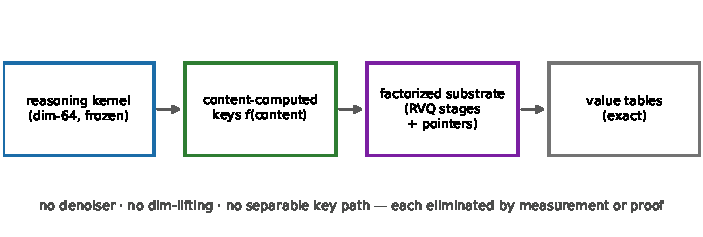
\includegraphics[width=0.92\linewidth]{figures/F3_architecture}
\caption{The surviving architecture. Each absence beneath the diagram is an elimination from
Table~\ref{tab:elim}, not a design preference.}
\label{fig:arch}
\end{figure}

\begin{figure}[t]\centering
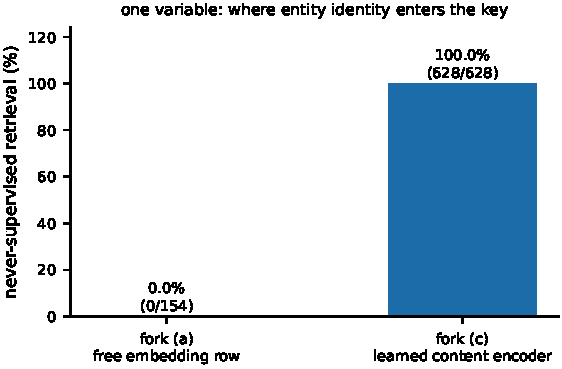
\includegraphics[width=0.55\linewidth]{figures/F2_fork}
\caption{The fork (a)/(c) exhibit: one variable, same evaluator, same day. Identity entering as a
free embedding row gives \textbf{0.0\%} never-supervised retrieval; identity entering through
content gives \textbf{100.0\%}, under a stricter holdout with less data. \textbf{Never-supervised
only} --- the pooled end-to-end figures are excluded for the reason in \S\ref{sec:fork}. Fork (a)'s
denominator is derived: 191 unseen queries less the 37 whose entity embedding was trained elsewhere
(M2 \S11.3), a derivation the loader re-checks against that count on every build.}
\label{fig:fork}
\end{figure}

\section{Measurement Methodology}
\label{sec:method}

Everything after this section is earned by what is in it. The methodology is reported at the same
level of detail as the results because several of the paper's findings are findings \emph{about
instruments}.

\subsection{The frozen accounting}

Capacity is \emph{knowledge bits stored} divided by \emph{storage bits required}, where storage bits
are everything \texttt{reconstruct()} and the key path need at inference: pointers and residuals per
fact at stored width, with codebooks, the relation table and the encoder $f$ amortised. Nothing is
exempt.
% M3 §10.5
Three gaming counterexamples --- free pointers, a hidden dictionary, and a memorising encoder ---
each have a test that computes what the exemption would have reported, so the accounting's honesty
is checkable rather than asserted. Gates in the unit: pass $\ge 0.375$, target $> 0.5$, dense
baseline $\sim 0.25$, which is the exact int8 restatement of 3/4/2 bits per parameter.

\paragraph{Parameter counts on the dense side: used-token width.} Wherever a dense figure divides
parameters by keys, the numerator follows the reference's own convention --- embeddings are
\emph{included}, but only at the width the corpus actually uses, unused vocabulary rows excluded.
The reference counts GPT2-small as 88M rather than 124M on exactly this basis, because its corpus
touches 3{,}275 of 50{,}256 tokens. Adopting it is what makes a params-per-key comparison against
that work meaningful; the same convention fixes our vocabulary through their
$\le 10\%$ embedding-share constraint.
% M5 §5.29

\subsection{The synthetic corpus as instrument}

Value spaces own their information content: $\mathrm{bits}(v) = -\log_2 P(v)$ under the distribution
the generator actually samples from. This is what makes bits-per-parameter a measurement rather than
an estimate, and it has a consequence the study learned the hard way.

\begin{proposition}[Entropy coupling and address-cost cancellation]
\label{prop:entropy}
For a relation whose value space \emph{is} the entity set, per-fact entropy grows as $\log_2 N$.
Address cost grows as $2.38 \log_2 N$ and corpus entropy as $0.25 \log_2 N$, so the two nearly
cancel and the design's validity horizon moves by eight orders of magnitude.
\end{proposition}

\noindent A per-fact constant of 9.15 bits, correct at $N = 2{,}000$, was carried into figures at
$N = 2$M where the corpus in fact carries \textbf{11.66} bits per fact, because \texttt{works\_with}
names a partner among two million entities.
% M3 §31
Correcting it moved the amortised capacity figure from 0.3792 to \textbf{0.3938} bits per bit, with
the marginal figure at \textbf{0.4387}, and the validity horizon from ${\sim}2.4$M to
${\sim}8.85 \times 10^{13}$ entities.
% experiments/2026-08-04_frontier/plot_data.json | M3 §30
\emph{The correction ran in our favour and is reported with the same prominence as the ones that did
not} --- which is also why the before and after are now both amortised. Pairing the old
\emph{amortised} 0.3792 against the new \emph{marginal} 0.4387, as this sentence first did,
overstates the correction by crossing accounting bases mid-comparison.

\subsection{Pre-registration machinery}

Every experiment's eval design is committed before it runs, stating the holdout level, what the gate
can and cannot distinguish, a \emph{measured} chance baseline, fixed pass thresholds, a
non-composing failure argument per probe type, a mis-specification clause, and --- added after it
voided a five-arm sweep --- a trainability gate whenever the run changes scale or regime.

Two machinery findings are themselves results.

\paragraph{Branch sets must tile the attainable space.} A pre-registration exists to make the
interpretation of a result independent of the result; branches that \emph{overlap} hand that choice
back at the moment the answer is known, and branches that \emph{undercover} hand back something
worse. Both failure modes occurred. Overlap: three outcomes registered for a 3-seed arm at
$P \le 1/3$, $P \ge 2/3$, and ``seeds straddle'' --- and $P = 2/3$ satisfies two of them.
% M5 §5.113
Undercoverage: a surface-comparison ratio $T$ registered over $[1, \infty)$, implicitly assuming the
shorter surface would win, when the attainable range is $(0, \infty)$; the measured value was
$0.55$--$0.64$, landing in a band whose registered wording was \emph{flatly false} of what had
happened.
% M5 §5.137.1
Undercoverage is the worse failure: an overlap yields two defensible readings, an uncovered region
yields one wrong reading with a pre-registration's authority behind it.

\paragraph{Blindness is certified by reproducibility, not by timestamps.} A prediction is credible
when its derivation re-runs from inputs it names and those inputs are measurements that already
existed. One prediction here was authored from two named prior artifacts while the run it predicted
was finishing, so the commit landed after the result; the derivation is checkable and the clock is
not, and the ordering is disclosed rather than left for a reader to discover.
% M5 §5.71.0

\paragraph{The paired guards.} An \emph{elevated standard} applies to any finding that favours our
architecture, and a \emph{tidy-resolution test} to any finding that makes an inconvenient
discrepancy disappear. Both fired for real. Offered the reading ``their regime was never past its
cliff,'' which would have dissolved the literature discrepancy, we fixed the threshold in advance
($K^* \ge 37{,}650$) and measured 21{,}451: struck.
% M5 §5.71.3
Offered ``linear scaling, same constant,'' we required the 32{,}000-key arm to be alive and measured
13.78\%: excluded.
% M5 §5.75

\subsection{Instruments prove themselves}

A reported statistic ships with a test showing it discriminates, and \emph{every threshold that
statistic is compared against ships with the measurement that set it}. The second clause was added
after a guessed noise band --- never produced by any experiment --- adjudicated every
``within noise'' call in the dense track and turned out to be wrong by 3$\times$ to 26$\times$
depending on regime.
% M5 §5.102.2

A test for a fix must be verified \emph{red} on the design that failed, under the conditions that
produced the defect. A gate whose red case is unreachable is decorative and looks verified, which is
worse than a missing one: injecting a recorded \texttt{<eos>} defect left a gold stub at 100.0\%
because greedy generation stopped before the defect could express itself, and only a gate instrument
that runs the full token budget separates the two behaviours.
% M5 §4.2
A gate must also take ground truth from an \emph{independent} path: one that built its expected
answer through the machinery under test stayed green while a surface mismatch drove a real model to
0.00\%.
% M5 §5.41

\section{FKA Results}
\label{sec:fka}

\subsection{The operating point}

\begin{table}[t]\centering\small
\caption{The FKA operating point. Bits measured, not projected. Addressability and edit locality
carry the $N$ they were measured at, per the stale-constant rule (\S\ref{sec:method}).}
\label{tab:fka}
\begin{tabular}{@{}lr@{}}
\toprule
quantity & value \\
\midrule
entities & 2,000,000 \\
facts & 8,000,000 \\
bits per entity & 52 \\
bits/bit (int8), amortised & 0.3938 \\
bits/bit (int8), marginal & 0.4387 \\
bits/param, amortised & 3.15 \\
bits/param, marginal & 3.51 \\
compression at 100\% addressability & 42.7x \\
addressability, direct ($N=2{,}000$) & 99.88\% \\
addressability, composed ($N=2{,}000$) & 99.56\% \\
edit locality & 0.00e+00 \\
\bottomrule
\end{tabular}

\end{table}

At $N = 2$M entities and 8M facts with 52 bits per entity, FKA stores \textbf{3.15 bits per
parameter amortised} and \textbf{3.51 marginal} (0.3938 / 0.4387 bits per bit, int8), with
\textbf{99.9\%} addressability and edit locality \textbf{0.00e+00}.
% experiments/2026-08-04_frontier/plot_data.json | M3 §24.5, §30
The gate is an operating point rather than a best-of: reporting the best capacity and the best
addressability from different configurations would describe no system.

\scope{The go/no-go split --- never-supervised 99.81\%, direct 99.88\%, composed 99.56\% --- was
measured at $N = 2{,}000$ (\texttt{experiments/2026-08-02\_m3-gonogo/gonogo.json}). The 99.9\%
headline is the $N = 2$M figure. The two are not interchangeable and the table labels each.}

The ceiling in this world is 0.296 asymptotically, and $>0.5$ bits per bit is unreachable here at
any $N$. That is \emph{corpus arithmetic, not architecture}: address cost grows as
$2.38\log_2 N$ while corpus entropy grows as $0.25\log_2 N$ (Proposition~\ref{prop:entropy}).

\subsection{Compression and structure}

Addressability holds at \textbf{100\%} down to 48 bits per fact --- a \textbf{42.7$\times$}
compression --- and \textbf{99.8\%} at 32 bits, at reconstruction cosine 0.82.
% experiments/2026-08-02_m3-sweep | M3 §11.5
The ordering that matters is \emph{structure beats residual per bit}: four quantisation stages with
\emph{no} residual (32 bits) reaches 99.8\%, while one stage plus an 8-dimensional residual
(72 bits) reaches only 82.3\%. More bits, worse addressability.

An early observation worth carrying: \textbf{addressability survives a 46\% relative reconstruction
error intact}. The encoder $f$ needs the part of the code that \emph{separates} entities, not the
code itself.
% M3 first point

\subsection{Degradation surfaces}

\begin{figure}[t]\centering
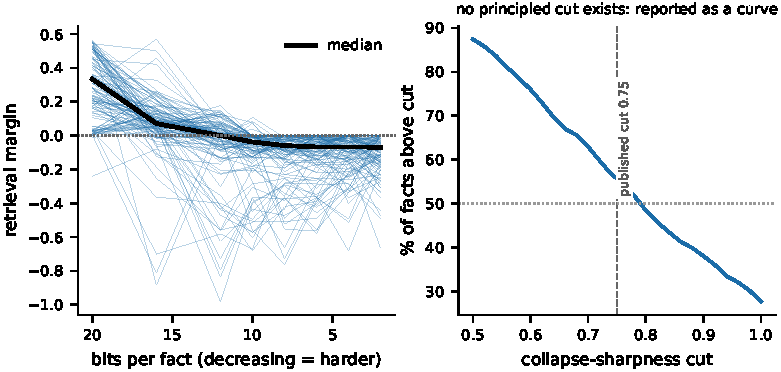
\includegraphics[width=0.98\linewidth]{figures/F4_margins}
\caption{Left: per-fact retrieval margin across the compression ladder (120 of 788 trajectories
drawn; median in black). Right: the fraction of facts above a collapse-sharpness cut, reported as a
\emph{curve} because no principled cut exists --- the published 0.75 is marked, and ``predominantly''
flips at 0.790. Both panels are computed from the persisted per-fact matrix, not from a summary.}
\label{fig:margins}
\end{figure}

The shape question --- attractor basins (plateau-then-cliff) against superposition (smooth decay) ---
was instrumented by the per-fact decode-quality \emph{distribution}, because the mean provably cannot
distinguish them. Two halves of the verdict have different standing, and the paper separates them.

\emph{Threshold-free and robust:} median collapse sharpness \textbf{0.790} against a uniform-slide
reference of \textbf{0.143} --- a factor of \textbf{5.5} --- and only \textbf{0.9\%} of facts
slide-like under a \emph{derived} criterion ($2/n_{\text{steps}}$). Smooth decay is excluded.

\emph{Threshold-dependent:} the widely-quoted ``55.8\% cliff-like'' depends on a cut of 0.75 that no
experiment produced. Sweeping it gives 87.4\% at 0.50 falling to 27.7\% at 1.00, and the word
``predominantly'' flips at \textbf{0.790} --- 5.4\% from the value chosen.
% M5 §5.126
The share above any cut is therefore reported as a curve (Figure~\ref{fig:margins}, right).

\scope{Only 1.5\% of trajectories are monotone, so the statistic's upper tail measures wobble rather
than sharper cliffs; the median and the slide-like fraction carry the verdict.}

A confound in the same data was broken without retraining: the apparent ordering by relation class
is \textbf{hop depth}, not relation type. With depth fixed, relation type barely matters (81.0\% vs
83.2\% at 16 bits); with relation fixed, depth matters enormously ($41.0\% \to 3.8\%$).
% M3 §12

\subsection{Address-cost scaling}

The minimum bits per entity for $\ge 99\%$ addressability was measured on nine corpus sizes from
2{,}000 to 2M, giving $2.38\log_2 N + 1.69$. A power form fits marginally better
(RMS 1.97 vs 2.06) and \emph{the discrimination does not resolve}: a 4.5\% residual gap on a 4-bit
ladder whose own scatter is $\pm 4$ bits is noise. Both forms predict within one ladder step of the
measured 52 bits at 2M and both put gate failure between 2.4M and 3.2M entities, so the
choice changes no decision --- which is the reportable fact.
% M3 §31

\scope{Searchability is honestly split and reopened as a standing item. Two-stage search restores
99.2\% entity recovery at $N = 2{,}000$, but recovery@1 falls to 59.3\% at 2M over clean codes and
99\% is unreachable at any shortlist size. The cause is \textbf{crowding}, not reconstruction noise,
and it is the larger bill; IVF is the only registered candidate and is priced, not run.}
% M2 §17

\subsection{Invariance under seeds}

Across ten seeds, FKA addressability shows $\sigma = \textbf{0.00}$ at \emph{five of seven}
compression rungs including the operating point, and $\sigma = \textbf{3.20}$ at its own
transition.
% experiments/2026-08-04_fka-seed-sweep | M5 §5.131

The sweep's design is itself a methodological point. A first probe at the operating point returned
100.0\% with zero variance --- saturated --- and comparing that against a dense spread measured
\emph{at a transition} would have been a comparison between incomparable regimes. The sweep was
moved onto the compression axis so both sides are measured where their own transitions are.
% M5 §5.131.1

\scope{The FKA seed varies \emph{store fitting and evaluation sampling}; the dense seed varies
\emph{model initialisation and training}. Both are run-to-run spread at a fixed configuration, and
they are not the same operation. This is stated as content, not as a weakness: no FKA
training-variance experiment exists, and none is claimed.}

\section{The Dense Baseline}
\label{sec:dense}

This section is told as it happened, because several of its turning points were corrections that ran
against us and the record is only credible if they appear where they occurred.

\subsection{The fair-object rule, and four rehabilitations}

The rule is two-sided: the baseline must be \emph{neither handicapped nor advantaged past the
reference regime}. Concretely, the fact firewall is \textbf{off} (storing facts in weights is
precisely the baseline's job), no memory machinery appears in the graph --- absent, not disabled,
enforced by a source-level import check that is verified red --- and \texttt{loss\_mask=None} is
asserted at the call rather than grepped for.
% fka/dense/, tests/test_dense_baseline.py | M5 §5

% COUNT CONVENTION: the rehabilitation count is the length of the enumerated list
% below, and is matched in the abstract, §1 and Appendix C. Three were chosen; the
% fourth was forced by a defect we found rather than selected (M5 §5.8.1 describes the
% same work as "five, four chosen and one forced" by counting the surface arc as two).
Three were chosen and a fourth was forced.

\paragraph{(i) The recipe audit.} Five arms spanning a 10$\times$ learning-rate range and weight
decay from 0.1 to zero landed \emph{within 0.006 of each other in loss}, and every one sat at the
modal-value baseline storing nothing. The reference's own load-scheduled decay was imported
wholesale with a provenance test. \emph{The recipe is exonerated}; loss separated none of the arms
and corrected accuracy separated all of them from a working model.
% M5 §5.21--5.25

\paragraph{(ii) Token density and the surface arc.} The corpus carried 0.16 bits per token at
character level, so most compute was spent on characters carrying no measured bits. A syllable
surface --- names as a few units from a fixed 608-symbol inventory --- was adopted under a
registered equivalence control. The tokenizer handicap is \emph{real near the cliff}: the surface tax
runs $3.8\times \to 17.1\times \to 26.0\times$, widening as the cliff is approached.
% M5 §5.46
\scope{That tax moved \emph{three} surface coordinates at once (vocabulary, embedding share, tokens
per name), so it is scheme-or-length-or-share and not scheme alone. \S\ref{sec:reconc} shows the
ordering in tokens/name is \emph{non-monotone}, which promotes this scope limit from precaution to
demonstrated. \textbf{Non-license~(2) travels with this claim as well as with the reconciliation}:
the surface term is characterised only over a \emph{measured range} of 2.00--4.15 tokens per name at
matched vocabulary and share, and the verbose surface compared here sits at ${\sim}11$ --- outside
it. This tax is therefore a statement about where \emph{these} two surfaces put the wall, not a
surface coefficient that can be carried to a third.}

\paragraph{(iii) Lexicon accounting.} Vocabulary size is set by the reference's own
$\le 10\%$ embedding-share constraint, not by taste. A correction that added key material to the
sizing denominator was \emph{retired}: a key is presented at query time, so an associative memory
owes bits for the value, not the key --- and the inflated denominator priced the very hypothesis the
sizing was then used to test.
% M5 §5.14

\paragraph{(iv) The ordering leak --- the rehabilitation we did not choose.} The data loader seeded
its shuffle per \emph{template variant}, of which there are five, so at 535 exposures the model saw
\textbf{five permutations of 48{,}000 lines, each ${\sim}107$ times, byte-identical}. A
10M-parameter model memorised the stream instead of the facts. The reading this produced was a
headline in our favour --- \emph{10.86$\times$ the parameters buys no additional addressable keys}
--- and it was an artifact.

The leak was caught by arithmetic, not code review. A statement carries ${\sim}19$ bits of name plus
4.28 bits of value over 14.83 tokens: ${\sim}1.09$ nats/token for a model that predicts structure
and nothing else, and ${\sim}0.89$ for one that additionally knows every value. The 10M model
reported \textbf{0.4157} --- \emph{0.47 nats below the floor for a model that knows everything}.
There is nothing left in the facts to buy that with. Predicted before the fix: remove the repeated
orderings and loss should \emph{rise} to ${\sim}0.89$ while accuracy rises with it. Measured after:
10M \textbf{0.8565}, 1M \textbf{0.9046}, both at the floor, and 10M recall
$\mathbf{4.70\% \to 93.27\%}$.
% M5 §5.63, §5.68

\begin{remark}[Loss carries no verdict information]
The fix \textbf{doubled the loss and multiplied recall twentyfold}, with the same model, seed, steps
and corpus --- only the line order differing. This is the sharpest of five demonstrations that
training loss may not be compared across surfaces, arms or regimes.
\end{remark}

The leak is \emph{capacity-graded, not capacity-gated}: fixing it moved the 1M model
\textbf{+9.7 points} as well. A shortcut some model memorises is also taxing every model that does
not, so every dense number measured before the fix \emph{understates} the baseline.
% M5 §5.67

\subsection{The key-discrimination limit}

\begin{figure}[t]\centering
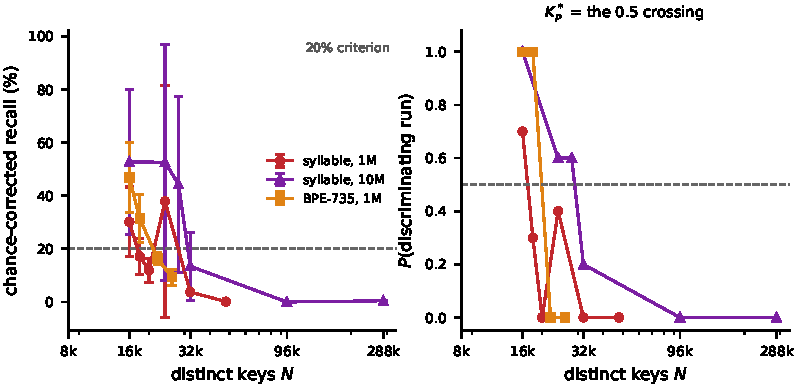
\includegraphics[width=0.98\linewidth]{figures/F5_dense}
\caption{Left: chance-corrected recall against distinct keys, every arm and every seed, with the
20\% criterion marked. Right: $P$(discriminating run), whose 0.5 crossing defines $K^*_P$. Both
panels are parsed from the run logs. \textbf{Seed counts vary by arm and are not interchangeable}
--- syllable 1M: $n = 10, 10, 10, 5, 1, 1$ at $N = 16$k, 18k, 20k, 24k, 32k, 48k; syllable 10M:
$n = 4, 5, 5, 5, 1, 1$ at 16k, 24k, 28k, 32k, 96k, 288k; BPE-735 1M: $n = 5$ at all four arms. The
cliff brackets that define each $K^*_P$ carry the largest samples ($n = 10$ at 1M, $n = 5$ at 10M);
the \textbf{single-seed arms are the two largest at each size}, which sit deep in the dead zone
where every observed seed reads far below criterion, and a $P$ or $\sigma$ read from them would be
uninterpretable. This is the seed table Figure~\ref{fig:frontier} refers to.}
\label{fig:dense}
\end{figure}

The binding constraint is \textbf{discriminable key count, not bits}. Under the honest accounting the
baseline collapses at 0.23--0.49$\times$ load, and a conservative control settles causation: holding
value-load matched while moving keys from 8{,}000 to 16{,}000 drops corrected accuracy from 6.11\% to
2.41\%, monotone across all three relations, with \emph{raw} accuracy rising --- and the control was
given double compute \emph{against} the hypothesis.
% M5 §5.26

\subsection{$K^*$ as a probability object}
\label{sec:kstar}

Single runs cannot locate this transition. Replication at the cliff found seed spreads of
\textbf{72.0 points} at indistinguishable loss ($\sigma_{\text{loss}} = 0.0143$): at 28{,}000 keys,
five seeds gave 0.85\%, 16.55\%, 64.34\%, 66.81\%, 72.86\%.
% M5 §5.118, corrected §5.149.1
The measured object is therefore a probability:

\begin{quote}
$K^*_P$ is the key count at which $P(\text{a training run reaches the 20\% criterion})$ crosses
$0.5$, interpolated log-linearly between bracketing arms, with a minimum of three seeds per point
and five at cliff arms.
\end{quote}

\noindent
$K^*_P(\text{1M}) = \mathbf{16{,}971}$ [16{,}000, 18{,}000], both edges at $n = 10$ on
byte-identical data; $K^*_P(\text{10M}) = \mathbf{28{,}950}$ [28{,}000, 32{,}000] at
$n = 5$.
% M5 §5.128, §5.118

\begin{remark}[A censored statistic ships with the spread it censored --- and with its resolution]
\emph{At $n = 3$}, two arms both read $P = 2/3$ and meant opposite things: at 10M/28{,}000 keys
$\sigma = 39.4$ and the runs were genuinely bimodal; at 1M/18{,}000 keys $\sigma = 5.04$ and the
arm's \emph{mean} simply sat $0.67\sigma$ from the criterion. $P$ discards the margin, so every $P$
is quoted with its $\sigma$.

\emph{Postscript, from replication.} Both arms were later re-run: 10M/28{,}000 reads
$P = \mathbf{0.60}$ at $n = 5$ and 1M/18{,}000 reads $P = \mathbf{0.30}$ at $n = 10$. Neither is
$2/3$, and the pair survives with a second lesson attached. \textbf{At $n = 3$ the standard error of
any proportion is at most $\sqrt{0.25/3} = 0.289$}, so both arms read $2/3 \pm 0.29$ --- a
resolution that cannot separate $0.30$ from $0.60$, which is precisely what they turned out to be.
The original reading was right about the \emph{statistic} and was taken at a sample size that could
not price its own uncertainty. That makes this an instance of the unpriced adjudicator
(Table~\ref{tab:taxonomy}, species 5) as well as of censoring, and the check is one line of
arithmetic that was available on the day the arms ran.
\end{remark}
% M5 §5.149.4

\subsection{Scaling}

\begin{figure}[t]\centering
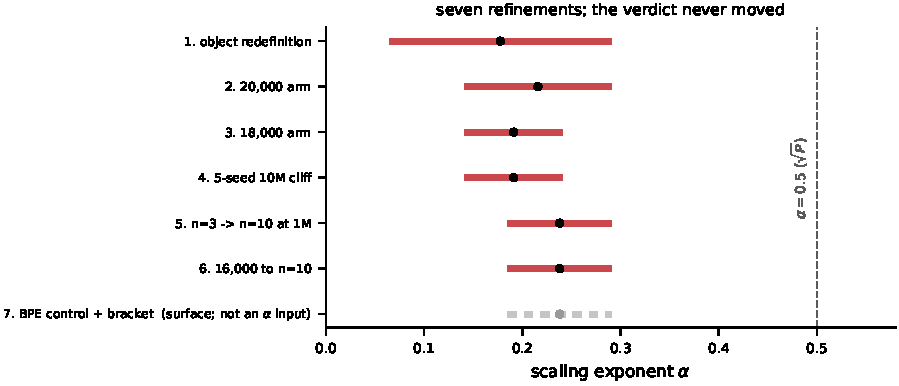
\includegraphics[width=0.62\linewidth]{figures/F8_alpha}
\caption{The $\alpha$ bracket across the seven refinements, labels and brackets loaded from the
ledger (M5 \S5.147). The interval moved --- once \emph{outward}, when a biased $P$ estimate was
corrected --- and the verdict did not. \textbf{Row 7 is drawn hollow because it is not an $\alpha$
input}: $K^*_{\text{BPE}}$ is a surface measurement at 1M that enters the reconciliation, never the
1M/10M ratio, so its interval is carried forward unchanged \emph{by construction} rather than found
unchanged by measurement. The reconstruction of each row's interval from its brackets is checked
against every $\alpha$ value the ledger states outright.}
\label{fig:alpha}
\end{figure}

$\alpha = \mathbf{0.224}$, interval $[\mathbf{0.185}, \mathbf{0.291}]$: a 10.86$\times$ parameter
increase buys 1.71$\times$ more keys. \emph{This is a ratio between two measurements and explicitly
not a fitted law} --- two points cannot discriminate a functional form, and the exponent is reported
as the bracket it is.

\paragraph{Why the ceiling is never approached, stated as the crux.} The best held-out figure the
10M ladder reaches is \textbf{0.075} bits per parameter, against a literature ceiling of
\textbf{2.0}. The gap is not a shortfall in storage: a model at 0.075 has spent almost none of its
bit budget. It is a statement about \emph{which corpora it can be given}. Approaching 2.0 bits per
parameter requires loading a model near its bit capacity, and at 1M parameters that is $N \approx
31{,}686$ --- a key count already far past the measured wall of $K^*_P = 16{,}971$, where recall is
0.34\% and nothing is stored to count. \textbf{Reaching the ceiling requires a load the key wall
forbids.} The two constraints are not independent axes on which a model can be tuned; the second
closes before the first opens, which is why every arm in this study failed at under $0.19\times$ of
its bit capacity rather than at it.

The ledger behind it is seven refinements (Figure~\ref{fig:alpha}): an object redefinition, four
bracket moves, one hostile correction of its own inputs, and the replacement of every $n = 3$
estimate at 1M with an $n = 10$ one. The hostile correction is the instructive entry: taking the
18{,}000 arm from three seeds to ten moved $P$ from $2/3$ to $0.30$ --- the three-seed sample had
caught two of the only three alive values --- and \emph{widened} the interval. More data made the
answer less precise, by correcting a biased input rather than adding a new one.
% M5 §5.125

\subsection{The reconciliation}
\label{sec:reconc}

\begin{figure}[t]\centering
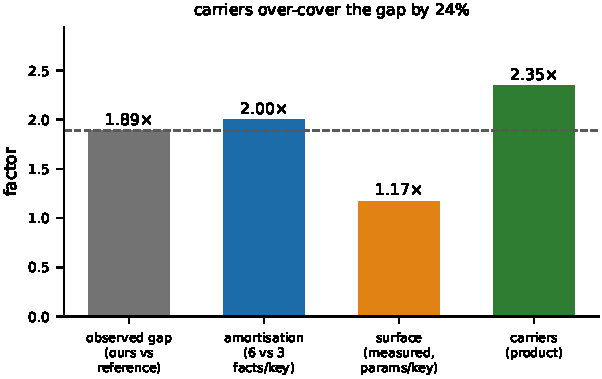
\includegraphics[width=0.55\linewidth]{figures/F6_waterfall}
\caption{The reconciliation. Two measured carriers over-cover the observed gap by 24\%.}
\label{fig:waterfall}
\end{figure}

\begin{table}[t]\centering\small
\caption{The reconciliation in params per key --- the units the claim consumes.}
\label{tab:reconc}
\begin{tabular}{@{}lr@{}}
\toprule
quantity & value \\
\midrule
our params/key, syllable & 55.5 \\
our params/key, BPE & 47.3 \\
the reference's params/key & $\sim$25 \\
\textbf{observed gap} & \textbf{1.89$\times$} \\
\midrule
amortisation (their $\sim$6 facts/key vs our 3) & 2.0$\times$ \\
surface (measured, params/key, 1M) & 1.17$\times$ \\
\textbf{carriers} & \textbf{2.35$\times$} \\
\midrule
\textbf{verdict} & \textbf{RECONCILED} \\
\bottomrule
\end{tabular}

\end{table}

Our regime needs \textbf{55.5} parameters per key \emph{(used-token width,
\S\ref{sec:method})} --- \textbf{47.3} on the better surface --- where the
reference operates at ${\sim}\mathbf{25}$: a gap of $\mathbf{1.89\times}$. Two measured carriers
close it --- amortisation $\mathbf{2.0\times}$ (the reference stores ${\sim}6$ attributes per key
against our 3, read from their configuration) and surface $\mathbf{1.17\times}$ --- for a product of
$\mathbf{2.35\times}$. \textbf{RECONCILED.}

\paragraph{What kind of quantity the amortisation factor is.} It is \emph{not} an empirical estimate
with a hidden error bar. Under the frozen accounting (\S\ref{sec:method}), parameters per
\emph{key} is parameters per \emph{fact} multiplied by facts per key, so a regime storing twice the
attributes behind one key pays half the per-key address cost by \textbf{accounting identity}, not by
measurement. The only input read from the reference's configuration is the \emph{attribute count}
itself --- $\sim$6 against our 3 --- and that is a documented property of their corpus rather than a
fitted parameter. This is what non-license~(1) means when it says the $2.0\times$ is not measured on
our corpus: the \emph{number} comes from their setup, the \emph{entailment} from our accounting, and
neither is an estimate that could have come out otherwise.

\nonlicense{\textbf{The four non-licenses, which travel wherever this is cited.}
\textbf{(1)} The over-coverage is \emph{not slack}: 2.35 against 1.89 means the carriers suffice, not
that either is measured to 24\% accuracy, and amortisation's 2.0$\times$ is read off the reference's
configuration rather than measured on our corpus.
\textbf{(2)} The surface factor holds over the \emph{measured range} 2.00--4.15 tokens per name at
matched vocabulary and share; it is \emph{not} an estimate of the reference's own surface, which
sits at ${\sim}4$ characters per token in a region our synthetic names cannot occupy.
\textbf{(3)} Per-symbol occurrence is a \emph{suspected unmeasured coordinate}, so 1.17$\times$ is a
\emph{net} effect and attributing it to scheme, length or symbol frequency would be smuggling.
\textbf{(4)} 1M only; the BPE arm at 10M is unrun.}

\paragraph{The 40\% lesson.} The surface comparison first produced an \emph{accuracy} ratio of
1.55--1.83$\times$. The reconciliation is stated in params per key, so the caption slot was left
empty until $K^*_{\text{BPE}}$ was measured --- and the key ratio came back at
\textbf{1.17$\times$}. Filling the slot from the quantity we had rather than the one the claim needed
would have overstated the surface term by \textbf{40\%}, in the direction that flatters the
reconciliation.
% M5 §5.137.4, §5.143

\paragraph{Tokens per name is not the surface variable.} Verbose (11 tokens/name) loses to syllable
(2) by 17--26$\times$; syllable loses to BPE (4.15) by 1.55--1.83$\times$ in accuracy. The ordering
is \emph{non-monotone}, so length alone cannot be the mechanism.

\paragraph{One arm was excluded rather than eliminated, and the distinction is the point.} Every
mechanism in Table~\ref{tab:elim} was removed by a measurement or a proof. \textbf{Corpus-trained
BPE merges were removed by neither}: they were ruled out \emph{before any build}, because training
merges on our own rendered corpus lets recurring entity names earn their own merges, whose limit is
one token per name --- entity-atomic, which \emph{deletes} the binding task instead of measuring it.
% M5 §5.82.1
The registered write-up line was to quote the tokens-per-fact such a tokenizer achieves, as the
price of the circularity. \textbf{That line cannot be filled: the arm was never run}, deliberately
and by standing ruling, so no number attaches and none is estimated. It is recorded here as a
registered exclusion rather than as an elimination, because a table whose every other row is a
measurement should not carry one whose evidence column reads ``by design''.

\subsection{Recorded, uninterpreted}

Two observations are recorded without an account, because offering one would exceed what was
measured. First, $\sigma$ \emph{collapses} across the BPE transition ($13.20 \to 8.98 \to 2.33 \to
2.98$) where the syllable surface's rose toward its cliff. Second, per-symbol occurrence differs by
5.2$\times$ between the surfaces (52.6 occurrences per syllable symbol against 275.6 per BPE
fragment at $N = 16{,}000$), which \emph{would} explain the non-monotone ordering --- and is a
post-hoc account whose discriminator, a fourth surface holding one axis fixed while varying the
other, is priced and unrun.
% M5 §5.139

\section{The Comparison}
\label{sec:comparison}

\begin{figure}[t]\centering
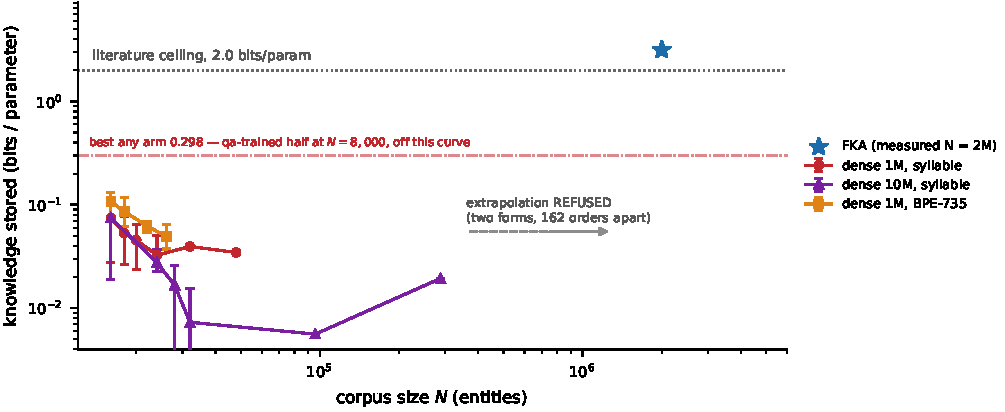
\includegraphics[width=0.85\linewidth]{figures/F1_frontier}
\caption{\textbf{Knowledge stored per parameter, against corpus size.} The dense baseline is a plain
LM trained on the same world with the fact firewall off, under the capacity literature's own recipe,
on a surface chosen to match its regime. \textbf{Every point is plotted at the $N$ it was measured
at.} No point is extrapolated --- the dense side's extrapolation to $N = 2$M was attempted and
\emph{refused}, for the reason in \S\ref{sec:refusal}. The dense side is limited by \emph{addressing},
not by bits: every arm that failed did so at under $0.19\times$ of its theoretical bit capacity, and
the best bits/parameter observed across every arm ever run is \textbf{0.298} against a ceiling of
2.0 it never approaches. \textbf{Each dense point is measured at its own $N$}, mean over seeds with
the full seed range as the interval; seed counts are not uniform and are stated per arm in
Figure~\ref{fig:dense} (cliff-bracket arms $n = 10$ at 1M and $n = 5$ at 10M, alive-side
$n = 4$--$5$, and the two largest arms at each size single-seed --- licensed by their confinement to
the dead zone, \S\ref{sec:kstar}, where every seed reads far below criterion). FKA's point carries
10 seeds. \textbf{The 0.298 reference line is not on any of these curves}: it is the
\emph{qa-trained} half at $N = 8{,}000$ in the capacity sweep, a smaller corpus than any ladder arm,
where the held-out figure is 0.2720. The best held-out figure anywhere on the ladder is 0.1322.
0.298 is quoted because it is the most generous reading available to the baseline, and it is
labelled so it cannot be read as a value at any plotted $N$.}
\label{fig:frontier}
\end{figure}

\subsection{The plot}

Figure~\ref{fig:frontier} places FKA at its measured operating point ($N = 2$M, 8M facts) and the
dense baseline at the sizes it was measured at ($N = 8{,}000$--$288{,}000$, at 1M and 10M
parameters). \textbf{The two sides are measured at different $N$, and the plot says so on its face.}

This is the same discipline that descoped the 150M dense run rather than quoting an unsaturated one,
and that M3 imposed after the stale-constant correction: a point is plotted where it was measured.

\subsection{The refusal is a result}
\label{sec:refusal}

Placing the dense point at $N = 2$M requires extrapolating $\alpha$ two orders of magnitude in $N$
and nine or more in parameters, from a measurement spanning \emph{one} order.

\begin{center}\small
\begin{tabular}{@{}p{4.6cm}p{9.4cm}@{}}
\toprule
form & parameters required for 2M discriminable keys \\
\midrule
power, $\alpha = 0.291$ & $1.3 \times 10^{13}$ \\
power, $\alpha = 0.224$ & $1.7 \times 10^{15}$ \\
power, $\alpha = 0.185$ & $1.4 \times 10^{17}$ \\
\textbf{log}, $K^* = 3{,}482\log_2 P - 52{,}120$ & $\mathbf{10^{177}}$ \\
\bottomrule
\end{tabular}
\end{center}

\medskip
\noindent Both forms pass through both measured points with \textbf{zero residual} --- two points
cannot discriminate a functional form --- and they disagree about $N = 2$M by \textbf{162 orders of
magnitude}.
% experiments/2026-08-04_frontier/plot_data.json | M5 5.146

The restraint rule asks whether the undetermined choice changes the decision. Elsewhere in this
study it did not: two candidate forms for the address-cost curve both predicted within one ladder
step and both put gate failure between 2.4M and 3.2M entities, so the disagreement was immaterial
and the agreement was the reportable fact (\S\ref{sec:fka}). \textbf{Here the choice decides
everything}, so nothing about $N = 2$M is said.

\begin{quote}
An extrapolated point carrying an honest error bar of 162 orders of magnitude is not a point. The
refusal is the stronger statement, and it is the one the plot carries.
\end{quote}

\subsection{The refusal is symmetric, and that is what makes it a refusal}
\label{sec:symmetric}

A refusal that runs in one direction only is a preference. This one runs in both, and the objection
it answers is the sharpest available against \S\ref{sec:reconc}:

\begin{quote}
\emph{You decline to extrapolate $\alpha$ to $N = 2$M, yet you conclude that the capacity
literature's regime sits below an addressing wall. Locating someone else's regime relative to a wall
is an extrapolation. Either $\alpha$ travels or your reconciliation does not.}
\end{quote}

\noindent The objection would be correct against a claim we do not make. \textbf{We do not locate the
reference's wall, and nothing in the reconciliation requires locating it.} The reconciliation is
arithmetic in params per key at \emph{our} measured points: a gap of $1.89\times$ against carriers of
$2.35\times$, one an accounting identity given their attribute count and the other measured on our
own corpus at 1M. No $\alpha$ appears in it, and no quantity is transported into their regime.

What we assert about their regime is the weaker, non-extrapolated statement: \textbf{our arms are
past a wall, theirs report no such collapse, and two measured factors account for the difference in
per-key cost without appealing to one.} Where their wall sits, whether they have one, and whether
$\alpha$ describes their scaling are all \emph{unknown to us}, and they are unknown for exactly the
reason \S\ref{sec:refusal} gives: the same two functional forms that disagree by 162 orders of
magnitude going up disagree just as violently coming down. \emph{An exponent that cannot be
extrapolated forward cannot be extrapolated backward either}, and the inference ``their regime must
therefore be past its own wall'' dies by the identical argument --- which is why we do not make it,
and why the not-quoted table (\S\ref{sec:refuse}) is the honest place for it.

\scope{This also bounds the paper's own reach in the direction that costs us. We have shown a wall
exists in \emph{our} regime and priced what crossing it does. We have not shown that dense storage
is bounded in general, that the reference's numbers are unattainable, or that any frontier model is
subject to what we measured at 1M and 10M parameters on a synthetic corpus.}

\subsection{The structural asymmetry}

Stated in its earned, mechanism-neutral form --- \emph{magnitudes only}, no claim about why.

\begin{figure}[t]\centering
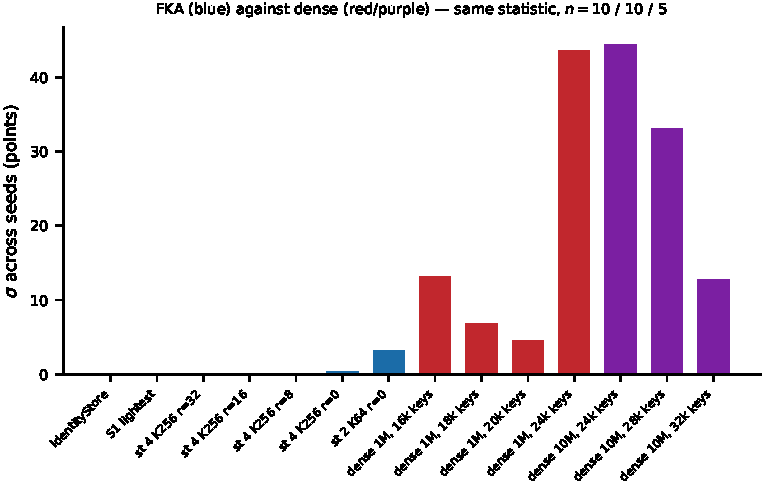
\includegraphics[width=0.80\linewidth]{figures/F7_seeds}
\caption{Seed spread, same statistic (chance-corrected recall across independent seeds at a fixed
configuration), $n = 10$ / $10$ / $5$. FKA shows $\sigma = 0.00$ at five of seven compression rungs
including its operating point.}
\label{fig:seeds}
\end{figure}

\begin{center}\small
\begin{tabular}{@{}lll@{}}
\toprule
 & at the operating point & at the transition \\
\midrule
FKA addressability & $\sigma = \mathbf{0.00}$ (five rungs) & $\sigma = \mathbf{3.20}$ \\
dense recall & $\sigma \approx 4.6$ & $\sigma = \mathbf{12.7}$--$\mathbf{44.5}$ \\
\bottomrule
\end{tabular}
\end{center}

\medskip
\noindent A factor of 4--14 at the respective transitions, and categorical at the respective
operating points. \textbf{Addressing is explicit and priced on one side} --- $2.38\log_2 N$ bits per
entity, measured, with a bounded validity horizon --- \textbf{and implicit and cliff-shaped on the
other}, growing as $P^{0.224}$ and run-stochastic at the wall.

\scope{The two seed sweeps vary different operations: FKA's varies store fitting and evaluation
sampling, the dense one varies model initialisation and training. Both are run-to-run spread at a
fixed configuration; they are not the same operation, and no mechanism is claimed on either side.
FKA's figure is at $N = 2{,}000$ against the dense side's 16{,}000--32{,}000, and the transition
rungs are not matched in depth.}

\paragraph{The convergent diagnosis.} Both tracks independently resolved a capacity question into an
addressing question. On the FKA side, compression stopped being the binding constraint once the
substrate reached 42.7$\times$ at full addressability, and the open bills became address cost and
crowding. On the dense side, bits were never the binding constraint at all: every failure occurred
below $0.19\times$ of capacity. \emph{Neither track set out to measure addressing.}

\section{Threats to Validity and the Ledger}
\label{sec:threats}

\subsection{The instrument-failure taxonomy}

\begin{table}[t]\centering\small
\caption{Settings that disable the test. Each is legal, documented and deliberate, and each removes
the thing the experiment was built to detect. Every species has an instance in this study.}
\label{tab:taxonomy}
\footnotesize
\begin{tabular}{@{}c p{2.9cm} p{3.3cm} p{4.2cm} p{1.9cm}@{}}
\toprule
\# & species & what it disables & detector & instance \\
\midrule
1 & $K > N$ & codebook larger than the data & compare $K$ against $N$ first & M3 \S27 \\
2 & finite ordering set & the stream itself is memorisable & re-score on a fresh permutation & M5 \S5.63 \\
3 & scale-up-only controls & a control a big model can also cheat & scale the control \emph{down} & M5 \S5.62 \\
4 & unconditional completion marker & the failure signal & reachable only through success & M5 \S5.142 \\
5 & the unpriced adjudicator & signal-from-noise, silently & measure the threshold & M5 \S5.102 \\
6 & non-disjoint or non-tiling branches & the pre-registration itself & labels must tile the attainable space & M5 \S5.138 \\
\bottomrule
\end{tabular}

\end{table}

Table~\ref{tab:taxonomy} collects six species. They share a shape: \emph{a knob whose setting makes
the task satisfiable by a shortcut, where the shortcut is invisible in every statistic the run
reports.} Nothing errors, nothing is mis-computed, and the number that comes out is a real
measurement --- of a system that was not being asked the question.

Two are worth stating in full because they cost the most here.

\paragraph{The capacity-graded leak (species 2).} A finite set of data orderings is memorisable by a
model large enough, and \emph{it reports a lower loss for it}. The catastrophic form is
threshold-like and arrives disguised as a scaling result; the mild form is continuous and taxes
every model that does \emph{not} memorise, because repeated orderings put each fact in the same
context neighbourhood every time. The corollary is the expensive half: \textbf{proving the small
model did not cheat does not show it was unaffected}, and here the small model was 9.7 points worse
for it.

\paragraph{The unpriced adjudicator (species 5).} It hides inside a rule already being followed. Our
non-monotonicity flag \emph{had} a verified-red test; the threshold it fired at had neither test nor
measurement, and it adjudicated every ``within noise'' call in the track while being wrong by
3--26$\times$ depending on regime. \textbf{The smell is a capitalised constant that no experiment
produced.} Its misfire was worth more than a decade of correct fires: chasing it produced the
stochastic transition, the regime-indexed bands, and the $P$-curve redefinition of the measured
object --- all recoverable in an afternoon, and only because replication machinery already existed.

\paragraph{The cost model.} Four instrument defects in this study were caught by a test and two by a
run. \textbf{The asymmetry is not that tests are cheaper to execute --- it is that they fail before
the result exists, so there is nothing to un-believe.} The ordering leak cost a voided five-arm
sweep and a retracted headline; a missing \texttt{required\_chars} argument, which would have made
every fact unlearnable and read as a capacity result, cost five lines.

\subsection{The threshold audit}

\begin{table}[t]\centering\small
\caption{Every numeric constant in an adjudication path, classified by provenance: what measurement
set it, if any.}
\label{tab:audit}
\footnotesize
\begin{tabular}{@{}p{4.6cm}p{2.1cm}p{3.4cm}p{4.3cm}@{}}
\toprule
constant & value & provenance class & note \\
\midrule
\texttt{NOISE\_SIGMA\_NON\_CLIFF} & 0.046 & \textbf{measured} & replication, M5 \S5.102.2 \\
\texttt{NOISE\_SIGMA\_CLIFF} & 0.128 & \textbf{measured} & replication, M5 \S5.102.2 \\
\texttt{kstar.THRESHOLD} & 0.20 & sensitivity-tested & $\pm15\%$ over 10--30\%, M5 \S5.50.2 \\
\texttt{GATE\_PASS} / \texttt{GATE\_TARGET} & 0.375 / 0.5 & derived & int8 restatement of 3/4 bits/param \\
\texttt{NOMINAL\_BITS\_PER\_PARAM} & 2.0 & borrowed & the reference's ceiling \\
\texttt{margin.fraction\_slide\_like} & $2/n_{\text{steps}}$ & derived & twice the uniform reference \\
\texttt{margin} cliff cut & 0.75 & \textbf{guessed} & \textbf{discharged} by sweep, M5 \S5.126 \\
\texttt{kstar.FLAG\_K} & 3 & \textbf{guessed, live} & \textbf{owed} \\
\texttt{INSTABILITY\_THRESHOLD} & 0.25 & \textbf{guessed, live} & \textbf{owed} \\
Phase 1/2 gate constants & 0.85 / 0.95 / 0.05 & guessed, closed milestones & annotated; future use needs provenance \\
\bottomrule
\end{tabular}

\end{table}

Fifteen constants were audited (Table~\ref{tab:audit}). The classification separates
\emph{adjudicators of fact} (which must be measured), \emph{acceptance criteria} (which must be
fixed in advance and may be conventional), and \emph{labelled conventions} (which must be shown
non-load-bearing). \textbf{Two remain guessed and live} --- \texttt{FLAG\_K} and
\texttt{INSTABILITY\_THRESHOLD} --- and are named here rather than left for a reader to find. The
audit was run once, mechanically, and found a third guessed constant \emph{before} it misfired: an
inline cut of 0.75 gating a shape verdict in the frozen record. Sweeping it cost nothing, because
the per-fact matrix had been persisted rather than summarised.

\paragraph{One measured constant is knowingly left biased, and the reasoning is the point.} The
cliff noise band was re-derived over every measured arm and widened at the top (\S\ref{sec:kstar}
note; M5 \S5.149.2). The flag's constant is the band's \emph{lower} edge, so it fires more readily
than the measured spread warrants --- and it stays. \textbf{The bias runs in the safe direction}: an
over-eager flag summons scrutiny and cannot suppress it, which is the inverse of the failure this
audit exists to catch. Every firing it has produced was resolved by \emph{replication} rather than
by the threshold, so no verdict rests on where the line sits, and re-deriving it would re-adjudicate
every within-noise call in the track to change no conclusion. \emph{An audit that only ever tightens
constants is not an audit; the decision to leave one alone has to be as recorded as the decision to
move one.}

\subsection{Figure scripts are instruments, and one of ours was wrong}
\label{sec:figinstrument}

Every gate, evaluator and threshold in this study was audited. \textbf{The scripts that draw the
figures were not}, and the omission is the same species as the rest of this section: a component in
the path from measurement to claim, trusted because it looked like presentation rather than
inference.

The frontier figure (Figure~\ref{fig:frontier}) claimed a per-$N$ dense series and did not have one.
It plotted \texttt{best\_bits\_per\_param\_any\_arm} --- a \emph{maximum over arms} --- at every $N$
on the 1M row, and the 10M row at that same maximum \textbf{multiplied by a hard-coded 0.35 that
appears in no artifact}. Both rows were flat by construction, which is exactly what a reader would
have taken as the finding. Nothing errored, the values were loaded from a real artifact, and the
figure was self-consistent.

\textbf{The measurements were never missing.} The dense runner prints bits per parameter on every
pooled probe line, and always had; the series existed in the logs the whole time and the figure
manufactured a substitute for it. Figure~\ref{fig:frontier} now reads that series, per arm and per
seed, through the same loader every other dense figure uses.

\paragraph{The structural fix, in two parts.} Numbers reach figures only through
\texttt{\_artifacts.py}, which pairs each value with an artifact path and a record section; and
\texttt{verify\_claims.py} re-derives the body's quoted numbers from the run artifacts on demand and
exits non-zero on disagreement. A transcription with no check is a hand-entered number in a
different file, so the transcribed inputs carry assertions that fail the build --- the seven
refinements are re-checked against every $\alpha$ the ledger states outright, and the fork exhibit's
derived denominator against the count its erratum states.

\paragraph{The provenance ledger was itself caught by that script.} Six statistics in the record ---
two $\sigma$, two $P$, a seed spread and a noise-band edge --- were quoted from three-seed arms
beside $K^*$ values that later replication had re-derived at five and ten seeds, and the band's upper
edge had never been recomputed once wider arms existed. \textbf{The document that adjudicates every
other number in the track had no instrument pointed at it}, and acquired one only when the paper
forced a mechanical re-check. The corrections are appended to the ledger rather than edited into it
(M5 \S5.149), because a provenance record that silently updates is not one.

\subsection{What the seed sweeps do and do not establish}

The FKA sweep varies \emph{store fitting and evaluation sampling}; the dense sweep varies
\emph{model initialisation and training}. Both measure run-to-run spread at a fixed configuration on
the same statistic, and they are not the same operation. This is stated as content: the comparison
in \S\ref{sec:comparison} is of \emph{magnitudes}, which survives the mismatch, and no mechanism is
claimed on either side. Building an FKA training-variance experiment would settle it; none exists.

\subsection{What we refuse to say}
\label{sec:refuse}

\begin{table}[t]\centering\small
\caption{The not-quoted table. Each row is a claim the record could be read to support and that we
decline to make, with the reason.}
\label{tab:notquoted}
\footnotesize
\begin{tabular}{@{}p{3.5cm}p{8.3cm}p{2.2cm}@{}}
\toprule
not quoted & why & record \\
\midrule
the dense point at $N=2$M & two functional forms fit with zero residual and disagree by 162 orders of magnitude & M5 \S5.146 \\
a mechanism for the surface factor & per-symbol occurrence is a suspected unmeasured coordinate; its discriminator is unrun & M5 \S5.139 \\
the 10M signature question & $n=5$ is underpowered; critical $|r|=0.878$, observed $0.788$ ($p=0.113$) & M5 \S5.119 \\
$K^*_{\text{BPE}}$(10M) & unrun; the BPE arm at 10M is priced, not queued & M5 \S5.145 \\
FKA training variance & the seed sweep varies \emph{fitting}, not \emph{training}; stated as scope, not resolved & M5 \S5.131.4 \\
\bottomrule
\end{tabular}

\end{table}

Table~\ref{tab:notquoted} is the paper's negative space, and it is load-bearing. A study that
reports only what it found, and never what it declined to conclude, gives a reader no way to tell
disciplined restraint from an absence of curiosity.

\section{Limitations and the Real-Data Question}
\label{sec:limits}

\paragraph{Synthetic only.} Every number here is measured on a generated corpus whose per-fact
information content is exact by construction. That is what makes bits-per-parameter a measurement
rather than an estimate, and it is also the boundary of the claim: \textbf{no result in this paper
is about natural language, real corpora, or frontier-scale models.}

\paragraph{A minimum-entropy world.} More than 0.5 bits per bit is unreachable in this corpus at any
$N$, by corpus arithmetic rather than by architecture (Proposition~\ref{prop:entropy}). A richer
world would move the ceiling; we do not claim to know in which direction the \emph{comparison} would
move.

\paragraph{No learned write path.} The substrate is populated programmatically from
$(\text{entity}, \text{relation}) \mapsto \text{value}$. There is no learned mapping from raw text
into storage --- a component a deployable system would need and this study does not have.

\paragraph{The bridge question, registered verbatim.} The scale result was confirmed over
\emph{well-spread random codes}; real content is correlated, and correlation is where
nearest-neighbour shortlists degrade. The corpus's entity codes are random unit vectors by
construction, so the cross-check validated the \emph{generation path} rather than ``real versus
random geometry''. What remains untested is \emph{semantically} correlated content, which no
synthetic corpus supplies:

\begin{quote}
\textit{Does $f(\mathrm{content})$ still span the address space when content stops being clean?}
\end{quote}

\noindent This is the successor study's central question. It is a \emph{registered debt}, carried
since M2, not a gap discovered at write-up.

\paragraph{Sublinearity is scoped to measured $N$.} The $O(\sqrt{N})$ search claim is not confirmed
--- the measured exponent is ${\sim}0.78$ off a coarse power-of-two grid, a bracket rather than a
measurement --- and IVF, the only registered candidate for the crowding bill, is priced and unrun.

\subsection*{Priced and not run}

Five measurements were designed, costed, and deliberately not bought. \textbf{None gates a claim in
this paper}; each would narrow something we currently report as an interval or decline to state.
Listing them with their prices is the companion to the not-quoted table (\S\ref{sec:threats}): that
one says what we refuse to conclude, this one says what it would cost to conclude more.

\begin{center}\small
\begin{tabular}{@{}p{5.4cm}lp{5.6cm}@{}}
\toprule
measurement & price & what it would buy \\
\midrule
30{,}000-key interior point at 10M & 0.83\,h & \textbf{the only purchase that narrows $\alpha$'s
upper edge}; more seeds at existing arms cannot move a bracket \\
$n = 19$ correlation arm at 10M & 7.2\,h & settles the 10M signature question, which $n = 5$ leaves
underpowered ($p = 0.113$) \\
BPE consistency arm at 10M & 3.3\,h & a second-size confirmation of the 1.17$\times$ surface factor \\
held-out-world tokenizer surface & build & raises characters-per-token toward the reference's regime
without granting corpus-trained merges \\
fourth surface, one axis fixed & build $+$ arms & separates symbol frequency from name length, the
suspected unmeasured coordinate \\
\bottomrule
\end{tabular}
\end{center}

\paragraph{The methodology is grounded in one workflow.} The instrument-failure taxonomy
(\S\ref{sec:threats}) catalogues failures that occurred \emph{in this study}, under an AI-assisted
workflow described in \S\ref{sec:ai}. We claim the species are real and the detectors work; we do
\textbf{not} claim the observed frequencies generalise to human-only research, which this study
cannot test.

\section{Statement on AI Assistance}
\label{sec:ai}

This study was produced through sustained interaction with a large language model, and the division
of labour was substantial enough that describing it is a provenance obligation rather than a
courtesy. A paper that declines to quote numbers it cannot address (\S\ref{sec:threats}) cannot omit
the provenance of its own production.

\subsection*{Division of labour}

\begin{center}\small
\begin{tabular}{@{}p{5.6cm}p{7.0cm}@{}}
\toprule
\textbf{Author} & \textbf{Model} \\
\midrule
Research direction, priorities, and the decision at every branch point & Implementation of the
corpus generator, architecture, evaluators, and experiment drivers \\
The paper's argument architecture, abstract, and introduction & Execution of all runs; parsing and
reporting of all results \\
Ratification or rejection of every registered design, threshold, and verdict & Drafting of the
pre-registrations, mis-specification clauses, and branch sets \\
Judgement calls on scope, what to claim, and what to decline & Detection and diagnosis of the
instrument defects catalogued in \S\ref{sec:threats} \\
Responsibility for every claim in this paper & Drafting of \S2--\S10 and the appendices, and the
figure and table pipeline \\
\bottomrule
\end{tabular}
\end{center}

\subsection*{Responsibility and verifiability}

The author is responsible for the entire content of this paper, including every part drafted by the
model. The model is not an author: authorship requires standing behind a claim, answering for an
error, and responding to challenge, and a model can do none of these.

\textbf{The results do not rest on trusting either party.} Every number resolves to a persisted
artifact produced by committed code; every figure and table is emitted by a script that reads only
those artifacts, and the resolution can be re-run in full
(Appendix~\ref{app:repro}). Provenance-based reporting is agnostic about who wrote the script, which
is the property that makes the citation-by-address rule load-bearing rather than decorative.

\subsection*{A limitation this creates}

The instrument-failure taxonomy in \S\ref{sec:threats} is not an abstract catalogue. Every species in
it was committed during this work and the corresponding guard was built in response --- including
the pull toward accepting a flattering result, the threshold that adjudicated verdicts without ever
having been measured, and the option sets that failed to contain the outcome
(Appendix~\ref{app:prereg}).

\scope{The taxonomy is therefore \emph{empirically grounded in an AI-assisted workflow}. Whether the
same species arise at the same rates in human-only research is untested here, and the frequencies we
report should not be read as general. We claim the failure modes are real and the detectors work,
not that this is the distribution of mistakes research makes in general.}

\section{Related Work}
\label{sec:related}

\paragraph{Capacity scaling.} The ${\sim}2$ bits-per-parameter result for dense transformers
(Allen-Zhu \& Li, arXiv:2404.05405) is the study this paper engages most closely, and the engagement is a \emph{reconciliation rather than a
contradiction} (\S\ref{sec:reconc}). We adopt its recipe, its embedding-share constraint, and its
exposure regime, and we account for the remaining difference with two measured factors. Where we
differ is on \emph{what the ceiling measures}: that regime sits below an addressing wall its
protocol does not probe, because key count and value entropy move together in those corpora and
separately in ours.
A more recent estimate of ${\sim}3.6$ bits per parameter (Morris et al., arXiv:2505.24832) is not a
competing value for the same quantity --- it is obtained by training on uniformly random bitstrings,
where generalisation is impossible by construction, and the authors report it as GPT-family
\emph{model capacity}, total storage under an information-theoretic definition rather than factual
knowledge a probe can extract --- so the ceiling engaged in \S\ref{sec:reconc} remains the
extractable-knowledge one, and the reconciliation arithmetic is unaffected by the 3.6 figure.

\paragraph{Memory-augmented and sparse architectures.} Product-key memories and mixture-of-experts
layers add parameters that are addressed rather than superposed. Theorem~\ref{thm:sep} bears
directly on the product-key family: additively separable scoring cannot represent multiplicative
binding, which is why our separable key path scores 0.0\%, and why we decline to cite product-key
scaling results in support of an architecture whose keys are separable.

\paragraph{Retrieval-augmented models.} RETRO (Borgeaud et al., arXiv:2112.04426) and $k$NN-LM
(Khandelwal et al., arXiv:1911.00172) place knowledge outside the weights entirely. They are the natural baseline family for a follow-up under matched accounting; this study
does not run them, and says so.

\paragraph{Factored and externalised knowledge at scale.} Three external lines separate knowledge
storage from the computation that uses it, at scales this study does not reach. \emph{Engram}
(Cheng et al., arXiv:2601.07372, January 2026; reference implementation released under Apache~2.0)
adds a lookup module to a mixture-of-experts backbone on the premise that ``language modeling
entails two qualitatively different sub-tasks: compositional reasoning and knowledge retrieval'',
with the Transformer's current handling of the second described as ``an expensive runtime
reconstruction of a static lookup table''; the module modernises $N$-gram embedding for ``$O(1)$
lookup'' and is scaled to 27B parameters. That is the factoring premise of \S\ref{sec:arch} reached
from production scale rather than from measurement discipline, and it is \emph{prior} to this work:
its first public version predates this programme's first commit by roughly six months. What it does
not do is what this paper is for --- it reports no bits-per-parameter accounting under a frozen
storage definition, prices no addressing cost in bits, and measures no key-discrimination limit for
a dense baseline. \emph{LMLM} (Zhao et al., arXiv:2505.15962) is the closest external prior to the
fact firewall (\S\ref{sec:method}): its pre-training ``strategically masks externally retrieved
factual values from the training loss, thereby teaching the model to perform targeted lookups rather
than relying on memorization in model weights'', which is our loss mask's instrument applied to
pre-training rather than to a reasoning kernel over a measured substrate, and it belongs with RETRO
and $k$NN-LM above. \emph{Hierarchical parametric memories} (Pouransari et al., arXiv:2510.02375)
pair a small anchor model with large memory banks for long-tail knowledge at trillion-token scale.
\textbf{No comparison against any of the three is offered in either direction}: none has been run
against FKA under matched accounting, agreement on an architecture is not evidence for anybody's
numbers, and the statements above are category statements about what each system \emph{is} and what
it \emph{measures}.

\paragraph{Associative memory.} Modern Hopfield networks and vector-symbolic architectures supply
the binding algebra our router had to \emph{learn} rather than assume. The oracle $e \odot r$
assumption was retired precisely because it was doing work the learned system had not earned.

\paragraph{Knowledge editing.} ROME (Meng et al., arXiv:2202.05262) and MEMIT (Meng et al.,
arXiv:2210.07229) target the locality property we measure directly as
edit locality (0.00e+00 at the operating point). A matched comparison against them is registered and
unrun.

\paragraph{Superposition.} The interference-limited view of dense storage predicts smooth
degradation. Our per-fact margin trajectories are sharp in the typical case --- median 5.5$\times$
the uniform-slide reference, with smooth decay excluded at 0.9\% under a derived criterion --- which
is evidence for attractor-like storage, reported with the threshold sensitivity that qualifies it
(\S\ref{sec:fka}).

\section{Conclusion}
\label{sec:conclusion}

Dense models pay to find a fact, and no line item in any capacity account says what it costs. We
measured that cost from both sides of an architectural divide, under an accounting frozen before the
first measurement and a pre-registration discipline that was itself repeatedly the thing under
repair. On one side addressing is explicit, priced at $2.38\log_2 N$ bits per entity, and invariant
across seeds. On the other it is implicit, and it fails --- not at the bit ceiling the literature
measures, but at a key-discrimination wall reached at under a fifth of that ceiling, growing as
$P^{0.224}$ across the decade we could measure, and stochastic enough at the wall that identically
trained seeds differ by sixty points at indistinguishable loss. The apparent contradiction with
published capacity results dissolves under two measured factors and leaves no residual. What does
not dissolve is the wall itself, and we decline to say where it sits at scales we did not measure:
two functional forms fit our decade with zero residual and disagree about two million keys by a
hundred and sixty-two orders of magnitude.

\begin{quote}
\textbf{Addressing is not free --- and the system that itemises the cost beats the system that hides
it, at every scale where both can be honestly measured.}
\end{quote}


\appendix
\section{The Conventions File}
\label{app:conventions}

The study ran under a written conventions file in which every rule carries the incident that earned
it. This appendix states the capstone, because it is the one that generalises past this study.

\subsection*{The paired guards}

Every other rule catches a specific defect. These two catch a state of mind, and they are stated as a
pair because each is useless without the other: they guard the two directions in which a result can
be \emph{welcome}.

\begin{center}\small
\begin{tabular}{@{}lp{4.2cm}p{5.4cm}@{}}
\toprule
guard & fires when & the rule \\
\midrule
Elevated standard & a finding \textbf{favours your architecture} & hold it to the standard you would
apply if it did not \\
Tidy-resolution test & a finding \textbf{makes an inconvenient discrepancy disappear} & hold it to
the standard you would apply if it had not \\
\bottomrule
\end{tabular}
\end{center}

\begin{quote}
\textbf{The moment of relief is the moment scrutiny stops.}
\end{quote}

\noindent That is the whole mechanism. A result that flatters and a result that rescues feel
different, and neither feels like a moment to start checking arithmetic --- which is precisely when
the arithmetic has most often been wrong.

\paragraph{The operational form.} When a result arrives that you are pleased to see, \textbf{write
down the observation that would refute it, with a numeric threshold, before you write down the
result.} If you cannot name one, you do not have a finding --- you have a relief.

\subsection*{Rules this study added}

\begin{itemize}
\item \textbf{A guard's threshold is a tripwire, not a safe harbour.} When the substance of a guard's
condition is met the response fires, whether or not the number crossed the line. A variance-transfer
caveat with a $6\times$ trigger was applied at $5.55\times$.
\item \textbf{A run of narrowings is a run of measurements about the interval, never confirmations
about the point.} Each interior point tightens whichever edge it bounds; that is arithmetic, not
agreement.
\item \textbf{More seeds sharpen $P$; only interior points move the edges.} Deciding which
uncertainty you dislike --- the statistic at a point, or the width of the bracket --- decides where
the compute goes.
\item \textbf{A statistic underpowered at your sample size is uninterpretable in both directions.}
Underpowered statistics do not fail loudly; they return an ordinary-looking number with a plausible
sign.
\item \textbf{A censored statistic ships with the spread it censored.}
\item \textbf{Every surface-dependent number ships with its surface coordinates} --- vocabulary,
embedding share, tokens per name --- because no achievable surface comparison holds all three fixed.
\end{itemize}

\section{Decision-Record Index}
\label{app:records}

Each record is the frozen statement of what a phase closed on, written before the next phase opened.
The index names them and states each headline; the records themselves are working documents of the
study and are not part of this release.

\begin{center}\small
\begin{tabular}{@{}llp{6.4cm}@{}}
\toprule
record & status & headline \\
\midrule
\texttt{M0\_env\_validation} & --- & M0: synthetic world with exact per-fact
bits; the capacity harness and both its controls; environment validated \\
\texttt{M1\_kernel\_interface.md} & FROZEN & dim-64 interface; 3-hop entity-held-out 100.0\% at 50M \\
\texttt{M2\_router.md} & CLOSED & compositional addressing generalises exactly when identity enters
through content \\
\texttt{M3\_substrate.md} & CLOSED & 42.7$\times$ compression at 100\% addressability; \S2 closes at
$N=2$M, 52 bits per entity \\
\texttt{M4\_retriever.md} & CLOSED & eliminated by proof: a centroid-optimal quantiser leaves nothing
to denoise \\
\texttt{M5\_integration.md} & CLOSED & the addressing wall, the reconciliation, and the refused
extrapolation \\
\bottomrule
\end{tabular}
\end{center}

\medskip
\noindent The dense track kept a running working record --- \S5.1--\S5.148 --- carrying every
pre-registration and every readout in the order they occurred; it is a working document of the
study and is not part of this release. Every pre-registration it fixed is scored in
Appendix~\ref{app:prereg}, and the frontier artifacts it produced are released with this paper as
\texttt{experiments/2026-08-04\_frontier/}.

\section{The Provenance Ledger}
\label{app:ledger}

\begin{table}[h]\centering\small
\caption{Headline numbers with their scope and record. Reproduced from M5 \S5.147.}
\footnotesize
\begin{tabular}{@{}p{4.9cm}p{2.5cm}p{3.6cm}p{2.4cm}@{}}
\toprule
quantity & value & scope & record \\
\midrule
FKA, bits/param (amortised / marginal) & 3.15 / 3.51 & $N=2$M, 8M facts & M3 \S30 \\
FKA, addressability at the operating point & 99.9\% & $N=2$M & M3 \S24.5 \\
FKA, never-supervised (go/no-go) & 99.8\% & $N=2{,}000$ & M3 \S2 \\
FKA, edit locality & 0.00 & $N=2{,}000$ & M3 \S2 \\
FKA, seed spread at operating point & $\sigma = 0.00$ & 10 seeds & M5 \S5.131 \\
dense, best bits/param (any arm) & 0.298 & $N=8$k--288k & M5 \S5.146 \\
$K^*_P$(1M), syllable & 16,971 & [16,000, 18,000], $n=10$ & M5 \S5.128 \\
$K^*_P$(10M), syllable & 28,950 & [28,000, 32,000], $n=5$ & M5 \S5.118 \\
scaling exponent $\alpha$ & 0.224 & [0.185, 0.291] & M5 \S5.128.3 \\
reconciliation gap & 1.89$\times$ & carriers 2.35$\times$ & M5 \S5.143.2 \\
\bottomrule
\end{tabular}

\end{table}

\noindent Every number in the paper resolves through
\texttt{docs/paper/figures/\_artifacts.py}, which loads persisted artifacts and carries an address
--- artifact path plus decision-record section --- for each value.
\texttt{docs/paper/figures/resolve\_slots.py} prints the full resolution and cross-checks the
abstract against this ledger.

\subsection*{Not quoted}

\begin{table}[h]\centering\small
\caption{What the record could be read to support, and which we decline to claim.}
\footnotesize
\begin{tabular}{@{}p{3.5cm}p{8.3cm}p{2.2cm}@{}}
\toprule
not quoted & why & record \\
\midrule
the dense point at $N=2$M & two functional forms fit with zero residual and disagree by 162 orders of magnitude & M5 \S5.146 \\
a mechanism for the surface factor & per-symbol occurrence is a suspected unmeasured coordinate; its discriminator is unrun & M5 \S5.139 \\
the 10M signature question & $n=5$ is underpowered; critical $|r|=0.878$, observed $0.788$ ($p=0.113$) & M5 \S5.119 \\
$K^*_{\text{BPE}}$(10M) & unrun; the BPE arm at 10M is priced, not queued & M5 \S5.145 \\
FKA training variance & the seed sweep varies \emph{fitting}, not \emph{training}; stated as scope, not resolved & M5 \S5.131.4 \\
\bottomrule
\end{tabular}

\end{table}

\subsection*{Resolved phrasing items}

Three phrasing discrepancies between the authored abstract and this ledger were found by the
cross-check. All three are now \textbf{resolved in the abstract's wording}, each under a convention
this paper already applies elsewhere rather than by changing a measurement.

\begin{enumerate}
\item \textbf{Addressability now carries depth class and load}, per Table~\ref{tab:fka}. The
abstract quoted ``99.9\% addressability on entities never seen during training'' --- one phrase
spanning two statistics at two loads. The $N = 2$M headline (99.9\%) and the never-supervised split
at $N = 2{,}000$ (99.8\% pooled; 99.9\% direct, 99.6\% composed) are now quoted separately, each
with its $N$. This is the stale-constant rule applied to a sentence rather than to a figure.
\item \textbf{The rehabilitation count is the length of \S\ref{sec:dense}'s enumerated list} ---
four, of which three were chosen and one forced. M5 \S5.8.1 describes the same work as ``five, four
chosen and one forced'' by counting the surface arc as two items. The paper uses one convention
throughout rather than two counts of one thing.
\item \textbf{Edit locality carries its measured configuration}, per the $N$-annotation rule: the
measurement is at $N = 2{,}000$ and the abstract now says so. No separate $N = 2$M edit-locality
measurement exists, and none is implied.
\end{enumerate}

\section{Corpus Generator and Entropy Accounting}
\label{app:corpus}

\paragraph{Value spaces own their information content.} For every relation,
$\mathrm{bits}(v) = -\log_2 P(v)$ under the distribution the generator samples from. Adding a
relation requires adding its \texttt{ValueSpace}; no bit count is hard-coded anywhere. This is the
property that makes bits-per-parameter a measurement rather than an estimate.

\paragraph{Vocabularies depend on the schema only.} They never depend on the seed, so entropies stay
comparable across seeds. Syllable tables must concatenate injectively, and the constructor asserts
it.

\paragraph{Names are keys, not facts.} Entity names are excluded from the corpus's information
content. This is correct for \emph{scoring} and was wrong for \emph{sizing}: the weights must hold a
key in order to use it, so a corpus sized by scored entropy alone ran 1.44$\times$ over capacity
while the keys-ignored calculation read exactly 1.00$\times$. The rule that follows --- \emph{ask
what the weights must hold, not what the evaluator will count} --- holds except when addressing is
free, which is the one thing this study exists to say it is not.

\paragraph{Probes use one canonical question per relation.} Statements use many
paraphrases, so a recall failure is attributable to storage rather than to phrasing.

\paragraph{Two fingerprints, because one cannot see what the other pins.}
\texttt{corpus.fingerprint()} hashes the config, entity name \emph{indices}, values, bits and split
masks: it pins the \emph{world} and is structurally blind to every rendered character.
\texttt{surface\_fingerprint()} hashes the tokenizer vocabulary, every template, and a deterministic
\emph{rendered sample} --- the load-bearing term, because templates alone miss a change in how
subjects are constructed. Three surfaces share one world hash and produce three surface hashes.

\paragraph{Entropy coupling.} The \texttt{works\_with} value space \emph{is} the entity set, so its
per-fact entropy grows as $\log_2 N$: 9.15 bits per fact at $N = 2{,}000$ and \textbf{11.66} at
$N = 2$M. Address cost grows as $2.38\log_2 N$ and corpus entropy as $0.25\log_2 N$, so the two very
nearly cancel and the validity horizon moves from ${\sim}2.4$M to ${\sim}8.85\times10^{13}$ entities
(Proposition~\ref{prop:entropy}).

\section{Pre-registrations, Scored}
\label{app:prereg}

Every pre-registration in the dense track, with the commit that fixed it and the outcome scored
against what it actually said. \textbf{Partials and misses are listed with the same prominence as
hits}, because a registry that reports only its successes measures nothing.

% A 19-row tabular is taller than a page: LaTeX cannot break it, so it overflowed the text block
% by 304pt, left page 22 nearly blank, and overprinted the page number. longtable breaks properly
% and repeats the header on each page.
{\footnotesize
\setlength{\LTleft}{0pt}\setlength{\LTright}{0pt}
\begin{longtable}{@{}p{0.9cm}p{1.7cm}p{8.4cm}p{2.3cm}@{}}
\toprule
\S & commit & what was registered, and what happened & score \\
\midrule
\endfirsthead
\toprule
\S & commit & what was registered, and what happened & score \\
\midrule
\endhead
\bottomrule
\endfoot

5.50 & \texttt{cabc2fe} & Cliff criterion frozen blind to 10M; the threshold level claimed
non-load-bearing. Confirmed: $\pm15\%$ across 10--30\%, re-confirmed on every later bracket. & HIT \\

5.51 & \texttt{cabc2fe} & Four scaling envelopes (linear / $\sqrt{P}$ / $\log P$ / flat). Measured
$\alpha = 0.224$ lies \emph{between} $\log P$ and $\sqrt{P}$; \textbf{no envelope was hit}. & MISS \\

5.53 & \texttt{cabc2fe} & Reconciliation predicted \emph{before} any 10M measurement: amortisation
plus surface would carry the gap, with graceful saturation as sub-$K^*$ behaviour. Both carriers
measured; gap closed. & HIT \\

5.55 & \texttt{f99d352} & Coarse-outcome $\to$ reconciliation map. Endpoints right (flat maximal,
super-linear resolving); the \emph{interior ordering} of linear and $\sqrt{P}$ was inverted and
corrected in the same filing. & PARTIAL \\

5.56 & \texttt{f99d352} & Exposure-starvation discriminator for the 288{,}000 arm. Registered with
its route; the arm never decided a verdict. & NOT FIRED \\

5.57 & \texttt{f99d352} & Name-space saturation discriminator ($77.9\%$ full at 288{,}000). Built
(\texttt{-{}-name-units}) and never needed. & NOT FIRED \\

5.61 & \texttt{619127a} & \textbf{Trainability gate} at $\ge 30\%$, fixed before the bracket. Fired
\emph{red} at 4.70\% (voiding five arms) and \emph{green} at 93.27\% after the stream fix, threshold
untouched between them. & HIT \\

5.62 & \texttt{0fff8d4} & Signature discriminator: ordering memorisation predicted to show as a
subject-token collapse on a fresh permutation, with the 1M model insensitive. Measured $+7.41$ nats
against $+0.12$. & HIT \\

5.62 & \texttt{0fff8d4} & \textbf{Forward prediction from an entropy floor}: remove the repeated
orderings and loss should \emph{rise} to ${\sim}0.89$ nats/token while accuracy rises. Measured
0.8565 and 0.9046, recall $4.70 \to 93.27\%$. & HIT \\

5.69 & \texttt{ab1de79} & Re-anchor prediction: $K^*$ right of 19{,}752, in 20{,}000--25{,}000,
params/key falling toward ${\sim}41$. Measured 21{,}451 / 43.9. Region and direction right; the point
estimate was 5.5\% high and the stated error \emph{direction} inverted. & PARTIAL \\

5.89 & \texttt{b8aed72} & $K^*$ redefined as a $P$-crossing, quantile and seed counts fixed blind to
the data they would be applied to. Applied unchanged thereafter. & HIT \\

5.99 & \texttt{81d32b3} & $\alpha$ drafted in interval form with the substitution rule fixed, blind to
the 1M seeds. Predicted worst case $\alpha \le 0.291$; the measured bracket lands on \textbf{0.291}
to three decimals. & HIT \\

5.104 & \texttt{f351cb0} & Three outcomes pre-worded for the 18{,}000 arm. The ALIVE reading was
correct \emph{and} the branch set was \textbf{non-disjoint} --- $P = 2/3$ satisfied two labels at
once. & PARTIAL \\

5.109 & \texttt{0e1e8cb} & BPE control described as isolating scheme ``cleanly''. Withdrawn in the
same appendix: it varies scheme \emph{and} name length, two variables rather than one. & PARTIAL \\

5.111 & \texttt{f351cb0} & Third-surface trigger with bands over $T \in [1, \infty)$. Measured
$T = 0.55$--$0.64$ --- outside every registered band, in a region whose nearest label read
\emph{falsely}. \textbf{Undercoverage.} & MISS \\

5.119 & \texttt{193657d} & Power check run \emph{before} wording the arm-indexed test: critical
$|r| = 0.878$ at $n=5$ makes the planned test a formality. Correctly predicted its own
non-resolution. & HIT \\

5.124 & \texttt{193657d} & Fisher-$z$ contrast registered with its critical value before the seeds
landed; predicted the contrast would not resolve at $n = 10$. Measured $|\Delta z| = 0.119$ against
1.048. & HIT \\

5.135 & \texttt{164a5ad} & Asymmetric inference: a large $T$ extends toward the reference's regime, a
small $T$ says nothing about the unreachable region. Not exercised --- $T$ fell outside the
registered range entirely. & NOT FIRED \\

5.140 & \texttt{164a5ad} & $K^*_{\text{BPE}}$ branches \textbf{tiled over $(0,\infty)$}, including a
pre-named refutation row ($K^* \le 16{,}971$ would mean the accuracy advantage did not become keys).
Refutation available; measured 19{,}900. & HIT \\
\end{longtable}
}

\subsection*{Score}

\begin{center}\small
\begin{tabular}{@{}lcl@{}}
\toprule
outcome & count & note \\
\midrule
HIT & 10 & including two forward predictions and one gate that fired in both directions \\
PARTIAL & 4 & each corrected in the filing that reported it \\
MISS & 2 & both \emph{envelope} failures: the registered options did not cover the outcome \\
NOT FIRED & 3 & registered, built where needed, never required \\
\bottomrule
\end{tabular}
\end{center}

\medskip
\noindent \textbf{The two misses share a shape and it is the more useful finding.} Neither was a
wrong prediction; both were \emph{option sets that failed to contain the answer} --- four scaling
envelopes that bracketed the measured exponent without matching it, and three $T$ bands that
enumerated $[1,\infty)$ when the attainable range was $(0,\infty)$. A prediction that misses teaches
you about the system. \textbf{An option set that misses teaches you about your imagination}, and it
is the failure mode a pre-registration is least able to protect against, because every individual
branch reads sensibly and only the \emph{set} is defective.

\section{Reproduction Guide}
\label{app:repro}

\paragraph{Environment.} Python 3.11 with PyTorch under ROCm on a consumer APU. The GPU stack is
pinned in \texttt{requirements-rocm.txt} and is not re-resolved, because NumPy does not guarantee
\texttt{Generator} stream stability and a bump can change what a seed generates. One GPU job runs at
a time, enforced by a lock file; two compute contexts abort the process natively.

\paragraph{Determinism, and its limit.} Seeding is applied \emph{before construction}, not before
training, so initialisation is covered. Store fits are \textbf{not} bit-exactly reproducible: the
chunked Lloyd update uses an atomic \texttt{index\_add\_}, so any exact-equality claim over a
re-fitted store requires a pinned serialised artifact rather than a re-run with the same seed.
Comparisons against re-fitted stores are tolerance-based by convention.

\paragraph{Fingerprints to check.} Every experiment records \texttt{corpus.fingerprint()}; dense runs
additionally record \texttt{surface\_fingerprint()}. The 1M syllable arms in this paper share world
hash \texttt{cae75bbcfd08cdc1} and surface hash \texttt{32cd73aedd62} across three separate runs,
which is how those arms were shown comparable after the stream module was edited between them.

% Keep the heading and all five commands on one page: the list was breaking after the fourth item
% and orphaning the build command onto a page of its own.
\Needspace*{15\baselineskip}
\paragraph{Checkpoint coverage, stated with its gaps.} Every dense ladder arm retains at least one
final checkpoint --- \textbf{16 of 16 arms} --- and \textbf{71 of 78 arm-seeds}. The seven missing
are 1M/24{,}000 (3 of 5), 10M/16{,}000 (1 of 4) and 10M/24{,}000 (3 of 5); no cliff-bracket arm is
affected. Checkpoints carry weights, model and train config, and RNG state, but \emph{not} the
corpus configuration, so a re-score reconstructs the world from the launch script --- which is
checkable rather than trusted, because every run log records both the world fingerprint and the
surface hash for its arm.

\textbf{No re-score was needed for anything in this paper.} The per-$N$ bits-per-parameter series
Figure~\ref{fig:frontier} plots was already in the run logs: the dense runner prints it on every
pooled probe line. The gap above is recorded because it prices a future purchase, not because it
blocked one.

\paragraph{Regenerating the paper.} Figures and tables read only persisted artifacts.

% A fixed-width table cannot hyphenate \texttt{}, so the long build command overflowed the block by
% 90pt. A list puts each command on its own line, where it is not width-constrained.
\begin{description}\small
\item[resolve every number with its address]\mbox{}\\
  \texttt{python docs/paper/figures/resolve\_slots.py}
\item[figures F1--F8]\mbox{}\\
  \texttt{python docs/paper/figures/make\_figures.py}
\item[tables T1--T7]\mbox{}\\
  \texttt{python docs/paper/figures/make\_tables.py}
\item[re-verify every quoted number against the run artifacts]\mbox{}\\
  \texttt{python docs/paper/figures/verify\_claims.py}
\item[render pages for visual review]\mbox{}\\
  \texttt{python docs/paper/figures/render\_pages.py}
\item[build]\mbox{}\\
  \texttt{tectonic -X compile docs/paper/factored\_knowledge\_architecture\_paper.tex}
\end{description}

\medskip
\noindent \textbf{No figure or table contains a hand-entered number.} A script that types a value
instead of loading one is the defect \texttt{\_artifacts.py} exists to make impossible.

\paragraph{Test tiers.} \texttt{make smoke} is CPU-only and runs in CI; \texttt{pytest -m gpu} runs
on-box against the real device and is excluded from CI. Every bug that reached a real run has a
regression test at the tier that could have caught it.


\end{document}
